\documentclass[12pt,authoryear]{elsarticle} 

%\usepackage[a4paper,left,hmargin=2cm,vmargin=2cm]{geometry} 

\usepackage{multirow}
\usepackage{setspace}
\usepackage{amsmath}
\usepackage{hyperref}
\usepackage{xcolor} 
\usepackage{subfig}             %
\usepackage[utf8]{inputenc}

\usepackage[left,modulo,pagewise]{lineno}
\modulolinenumbers[3]

\journal{Ecological Informatics}

\definecolor{azulino}{rgb}{0.25,0.50 ,0.75} 
\usepackage{blindtext}

\hypersetup{
  bookmarksopen=true,
  pdftitle="Spatial and temporal representation of marine fish occurrences available online",
  pdfauthor=" ", 
  pdfsubject="Diversity and Ecoinformatics", 
  pdftoolbar=true, % toolbar hidden
  pdfmenubar=true, %menubar shown
  pdfhighlight=/O, %effect of clicking on a link
  colorlinks=true, %couleurs sur les liens hypertextes
  pdfpagemode=UseNone, %aucun mode de page
  pdfpagelayout=SinglePage, %ouverture en simple page
  pdffitwindow=true, %pages ouvertes entierement dans toute la fenetre
  linkcolor=azulino, %couleur des liens hypertextes internes
  citecolor=azulino, %couleur des liens pour les citations
  urlcolor=azulino %couleur des liens pour les url
}

\makeatletter
\renewcommand{\figurename}{\sf \textbf{Fig.}}
\renewcommand{\thefigure}{\arabic{figure}}
\renewcommand{\fnum@figure}{\sf\textbf{\figurename}~\textbf{\thefigure}}
\renewcommand{\tablename}{\sf\textbf{Table}}
\renewcommand{\thetable}{\arabic{table}}
\renewcommand{\fnum@table}{\sf\textbf{\tablename}~\textbf{\thetable}}
\makeatother

%%%%%%%%%%%%%%%%%%%%%%%%
%%%%%%%%%%%%%%%%%%%%%%%%
  \listfiles

  
\begin{document}

\begin{frontmatter}

  \title{
    Spatial and temporal representation of marine fish occurrences available online
  } 
  \author[ecoinfo]{Vanessa Pizarro}
  \author[ecoinfo,uach]{Andrea G. Castillo}
  \author[icml,FONDAP,COPAS,BASE]{Andrea Pi\~nones}
  \author[ecoinfo,iscv]{Horacio Samaniego\corref{corrauthor}}
  \ead{horacio@ecoinformatica.cl}

  \address[ecoinfo]{Laboratorio de Ecoinform\'atica, Instituto de Conservación, Biodiversidad y Territorio, Universidad Austral de Chile, Valdivia, Chile}

  \address [uach] {Programa de Doctorado en Ciencias mención Ecología y Evolución, Escuela de Graduados, Facultad de Ciencias, Universidad Austral de Chile, Valdivia, Chile}
  \address[icml] {Instituto de Ciencias Marinas y Limnológicas, Facultad de Ciencias, Universidad Austral de Chile, Valdivia, Chile}
  \address[FONDAP]{Centro FONDAP de Investigación en Dinámica de Ecosistemas Marinos de Altas Latitudes (IDEAL), Valdivia, Chile}
  \address[COPAS]{Centro de Investigaci\'on Oceanogr\'afica COPAS-COASTAL, Universidad de Concepci\'on, Chile}
  \address[BASE]{Millenium Institute Biodiversity of Antarctic and Subantarctic Ecosystems - BASE, Chile}
  \address[iscv]{Instituto de Sistemas Complejos de Valpara\'iso, Subida Artiller\'ia 470, Valpara\'iso, Chile}
  \cortext[corrauthor]{Corresponding author}


\linenumbers
\singlespacing

\begin{abstract} 

Despite the 243,000 species of  marine species described by 2022, our knowledge about the oceanic biodiversity is still incomplete. This knowledge gap carries potentially adverse and far-reaching consequences for the preservation of marine ecosystems, particularly in the context of the ongoing human-induced alterations to our biosphere and the rapid progression of climate change and global environmental shifts.

However, a large number of online repositories cataloging, storing and distributing biodiversity information hosting taxonomic information and species occurrence data have emerged recently. FishBase, the Global Biodiversity Information Facility (GBIF) and the Ocean Biodiversity Information System (OBIS) are part of these publicly available repositories  representing a variety of sources that have exploded in number. However, despite the incredible accumulation of biodiversity records, not all the information is really useful, nor does it represent any new knowledge regarding global species richness patterns.

In this study, we assessed the spatial and temporal representativeness of marine fish records (order Actinopterygii) found in the GBIF and OBIS global repositories. We have developed a methodological framework that relies on a series of non-parametric estimators for computing species richness from incidence data. This methodology employs hexagonal grids as sampling units that overlay marine bioregions across the globe.

Using standard ecological and spatial analysis tools, we identify regions that are adequately represented in terms of available records and therefore have more reliable data, as well as regions with few records that do not represent current species richness. We overlap these results with the location of marine protected areas and fishing exploitation zones to understand the anthropogenic effect on marine ichthyofauna. We additionally evaluate hypotheses regarding the taxonomic, geographic, and temporal distribution of information biases to deepen our current understanding of public records of species occurrences worldwide.

Considering that more than 40 years of information was analyzed, the results showed that on a global scale, the primary data on marine fish available on GBIF and OBIS platforms are still far from being representative and complete. Only 1.14\% of the records were useful for our analyses. In addition, we found that the information seems to be biased towards coastal areas, regions close to developed countries and areas where there is a large fishing activity. Finally, the best represented species and families are those with a small body size, which use shallow habitats and are usually recognized as having commercial, or cultural,  value.
  
\end{abstract}

\begin{keyword}
Ecoinformatics \sep Ecological Information Biases \sep Marine Fish \sep   Spatial and Temporal Representativeness \sep Species Richness
\end{keyword}

\end{frontmatter}
% \doublespacing
\onehalfspacing
\linenumbers
\section{Introduction}

Currently, the more than 243,000 species included in the World Register of Marine Species database \citep{worms2022} suggests that only 11 to 78\% of all marine species have been discovered, revealing a striking picture of vastly incomplete knowledge that may have serious implications for marine conservation \citep{luypaert2020}.
Moreover, ongoing climate change represents one of the greatest threats to biodiversity \citep{malhi2020climate, turner2020climate} and has already been documented to modify the distribution of marine species \citep{lenoir2020species}. Some of the described effects includes the invasion of non-native species leading to massive species turnover that may lead to the local extinction of large proportions of species \citep{cheung2009}. 

It is crucial to recognize that species richness, while being a diversity metric among many, is, in itself, an aggregate variable quantifying the end result of the splitting and lumping of the tree of life as a product of evolutionary processes \citep{Marquet2004}. Consequently, numerous endeavors have been directed towards the development of more comprehensive diversity indices, giving rise to significant scientific literature, aimed at describing ecological heterogeneity \citep{tuomisto_commentary_2011, moreno_commentary_2011, daly_ecological_2018}. However, within this literature, there appears to be a shifting focus towards examining the ramifications of biodiversity loss. This shift involves the adoption of new terminology designed to provide pragmatic concepts, such as ``species inventory'', ``taxonomic inventory'', or ``inventory completeness'', which are intended to convey more precise messages to policymakers, summarizing the richness of biodiversity \citep{pereira_essential_2013, butchart_global_2010}. Nevertheless, while the scientific community engages in debates over the use of biodiversity terminology, it is important to note that species richness continues to offer a concise and easily manageable description of variability across various other parameters characterizing the biota in both spatial and temporal dimensions \citep{APPELTANS2012}. Species richness remains an essential feature for comprehending how diversity evolves in response to natural and anthropogenic influences within biomes, regions, and ecosystems \citep{troia2017, magurran2011}.

Likewise, biodiversity can also be assessed through life history traits, which are modulated by both evolutionary factors and the variation in habitats and ecosystems \citep{neigel_book_1997, hutchings2005measuring}. We now know that biodiversity is more likely an expression of the heterogeneity of such life history traits. \citealt{alo2021macroecology}, for example, shows that while some of the fish diversity is certainly due to environmental processes, a large fraction of such richness variance is also determined by evolved life history traits related, for example, to migratory habits. Therefore, evaluating how life history traits impact richness metrics should deepen our understanding of fish diversity patterns.

While still short of having a robust and standardized biodiversity infrastructure \citep{heberling_data_2021}, a great diversity of online repositories with taxonomic information and species occurrences data exist. Among the most important databases hosting marine information are FishBase, a platform that hosts information on the taxonomy of fish, their ecology, trophic information, habitat and history of uses dating back to more than 250 years \citep{froese2000fishbase}; the Global Biodiversity Information Facility (GBIF), a platform that stores and allows for the free access to species occurrence records from around the world. GBIF is currently one of the repositories hosting the largest amount of such data in the world \citep{telenius2011, gbif}; and finally Ocean Biodiversity Information System (OBIS), which houses data on the occurrence and abundance of species from exclusively marine environments \citep{obis}. Records entered in these repositories are often used for research related to biodiversity assessment, taxonomic reviews, red listing of threatened species, species distribution, and generation of ecological niche models, among others \citep{yesson2007}. GBIF currently offers more than 1.62 billion occurrence records and OBIS more than 63 million, which increase considerably each year \citep{gbif, obis}.

The records of both platforms come from a wide variety of sources collected following different methodologies at different temporal and spatial scales introducing a great variety  biases \citep{beck2014, zizka2020}. Among these, three main types of biases have been described: (i) taxonomic, this occurs when some species and/or families are better sampled than other rarer species \citep{chandler2017}; (ii) geographic, when data input is unevenly distributed across geographic regions and may prove to obscure inter-region comparisons \citep{yang2013geographical, yesson2007}; and (iii) temporal, which may be prevalent when comparing different time periods as data coverage is unevenly distributed over time \citep{chandler2017, yang2013geographical}. While these biases introduce some uncertainty regarding reliability of species richness descriptions obtained from online platforms \citep{beck2014, garcia2015}, they have largely been used to provide an extensive overview of macro-ecological patterns of distribution not available otherwise \citep{mora2008completeness,troia2017}. 

Still, identifying how sampling effort is distributed across space and time is a necessary step to interpret biodiversity patterns and reduce biases as understanding the distribution of our biota is essential to design protection efforts. This may be achieved through different weighting schemes for records in areas with sufficient sampling that provide a more reliable contribution compared to underrepresented regions \citep{phillips2009, hortal2008, yang2013geographical}. 

We here assessed the spatial and temporal representativeness of marine fish records available in the global GBIF and OBIS repositories at the level of marine bioregions in order to pinpoint the location of records that best quantify the diversity of marine fishes. The result is a spatial representativeness analysis that we then overlay on marine conservation areas \citep{wcmc2022} and fisheries exploitation areas \citep{fao2014} to learn whether marine conservation efforts, as well as large fisheries, are located in areas of high species richness or in areas of insufficient data coverage. 

Finally, we also analyzed the potential effect that some attributes could have on the incidence of more records in global database repositories. Specifically, we evaluated three research questions related to how body size, habitat depth and commercial use relates to the representation of marine fish occurrences. We ask whether a better representation in the online platforms may be due to the over sampling of larger fish, caused by its easy identification; that shallow areas provide easy access to sampling; and economic and commercial interest have elicit a larger representation of culturally relevant species among online biodiversity repositories.  

\section{Methods}
\subsection{Species data}
\label{sec:spp-data}

We use all recorded ocurrences from the order Actinopterygii hosted in GBIF and OBIS repositories \citep{GBIFdata,OBISdata}. Following \cite{alo2021macroecology}, evolutionarily older taxa, such as Cephalaspidomorphi, were excluded from this analysis. The libraries \textit{rgbif} and \textit{robis} of the statistical package R were used for data extraction \citep{chamberlain2017, provoost2020, rcore2018}.
%
Both repositories have collaborated since 2001, sharing data on the co-occurrence of marine life \citep{OBISdata}.
Nevertheless, recent investigations have shown significant disparities in data contributions, revealing notably low percentages of shared data \citep{chollettComparingBiodiversityDatabases2020,moudryQualityUsabilityChallenges2020}. Noteworthy distinctions exist between the two platforms, encompassing diverse data sources and methodologies, along with substantial variations in temporal and spatial scales associated with data collection \citep{zizka2020}. Due to these disparities, scholars recommend a meticulous examination and refinement of these data repositories \citep{bonnet-lebrunOpportunitiesLimitationsLarge2023}. To enhance the quality and reliability of the information, a comprehensive series of filters has been systematically applied in our analysis. To minimize errors associated with the public usage of GBIF and OBIS repositories, we curated the dataset following \cite{zizka2020} and filtered the dataset by the columns labeled ``scientific name'', ``family'', ``year'', ``Longitude'' and ``Latitude''. We retained all taxonomic information down to the species level and removed records with \texttt{NA} in these columns. We also removed any duplicated record with identical latitude and longitude as well as any record collected before 1980 \citep[see][]{alo2021macroecology,garcia2015}. Each record was further assigned to a marine bioregion following  \cite{costello2017marine}. Spatial data manipulation and plotting was performed with the aid of the following libraries: \textit{sf}, \textit{dplyr}, and \textit{cartography} \citep{giraud2016cartography, pebesma2018simple, wickham2021dplyr}. We finally labeled and removed any exotic species record using the \texttt{distribution()} function provided by the \textit{rfishbase} library \citep{boettiger2012rfishbase, froese2021fishbase}. To limit our analysis to species occurring within their native range each record was checked against the classification of FAO fisheries area for consistency \citep{fao2014}. A summary of the number of records is provided in \ref{sec:appDB}.


\subsection{Data Analysis by Bioregion}
\label{sec:data-analysis}
Once the database was cleaned, a subset of the data was extracted for each of the 30 bioregions. For each bioregion, a count of records, species and families was made, and the Shannon diversity index was calculated using the \textit{vegan} library in R \citep{vegan}.

\subsubsection{Spatial Representativeness Analysis}
\label{sec:spat-repr-analys}
To assess the spatial representativeness of the data, bioregions were gridded into hexagonal cells of equal area to maximize fit to bioregions areas using a cylindrical equal area projection  (i.e. EPSG Code:54034). We approximated 1$^{\circ} \times$ 1$^{\circ}$ hexagonal lattice by computing cells of $10^4$ square-kilometers, resulting in a total of  57,067 cells. In the appendix, we evaluated two additional spatial resolutions: 5$^\circ$ and $10^\circ$ lattice with a total of 3,029 and 953 cells respectively using a gridcell of $2.5\times 10^5$, and $10^7$ square-kilometers in order to analyze different biodiversity macropatterns \citep{tittensor2010global}. The expected species richness ($S_{exp}$) was computed as the mean between three non-parametric richness estimators: Chao2 ($S_{chao}$), Bootstrap ($S_{bootstrap}$) and Jackknife 1 ($S_{jackknife1}$) \citep[see][for individual definition of indices]{magurran2011}. Such averaging seeks to minimize biases and potential errors of under- or over-estimation by using a single richness estimator following the work of \citep{mora2008completeness, troia2017}.

We then produced a species representativeness index (SRI) by comparing the observed richness ($S_{obs}$) per cell to $S_{exp}$ \citep{troia2017}, $SRI_i = \frac{S_{obs}}{S_{exp}}$. This is an undersampling index that indicates the degree of representativeness of records to quantify the actual species richness in each cell ($i$). Its value ranges from 0 to 1, where 0 represents an unsampled cell and 1 represents a fully sampled one.



The Species Richness Index (SRI) is employed as a metric to assess the accuracy of databases in depicting actual species richness. Consequently, we propose a systematic categorization of cells into three classes — ``low'', ``medium'' and ``high'' — based on the frequency distribution of SRI, as illustrated in Fig. \ref{fig:SRI_hist}. Cells with only one record are identified as having insufficient records (IR) for estimating S$_{est}$. Those with an SRI in the range (0, 0.60) are categorized as ``low'', while those falling within the interval (0.60, 0.85) may be characterized as possessing a ``medium'' level of representativeness. Furthermore, cells within the range (0.85, 1.00) are identified as ``high'', signifying an adequate representation of species diversity. Maps illustrating the raw values for observed species richness (S$_{obs}$), expected species richness (S$_{exp}$), and SRI are provided in Fig. \ref{fig:S+So+Es}.


\subsubsection{Temporal Representativeness Analysis}
\label{sec:temp-repr-analys}

We constructed species accumulation curves, employing years as the units of sampling, to examine the temporal distribution of data records within each bioregion. To assess the adequacy of the sample, we focused on the last four years of data (2016-2020), representing the final 10\% of each accumulation curve. We employed a linear fit following the rescaling of the SRI to facilitate statistically comparable slope measurements. Slopes approaching zero suggest bioregions that have been adequately sampled, whereas slopes deviating from zero indicate insufficient sampling efforts over time.

\subsubsection{Gap Analysis}
\label{sec:gap-analysis}
We overlaid the spatial representativeness map (\S \ref{sec:spat-repr-analys}) with shapefiles of Marine Protected Areas (MPA) \citep{wcmc2022} and fishing exploitation areas reported by \citep{fao2014}. The superposition of these layers allowed us to calculate the extent of protection offered by MPA for each  bioregions on a cell basis, and the extent of cells in designated fishing zones. This exercise allows to jointly assess the relationship between two opposing human impacts and current uncertainties about marine fish diversity. 

\subsubsection{Bias Assessment}
\label{sec:bias-assessment}
The evaluation of potential biases generated by body size, habitat depth and cultural value of species (\S \ref{sec:spp-data}) was assessed from the fishbase database \citep{froese2021fishbase}. We generated a frequency distribution plot for the reported length of each species in the database, employing equal intervals of 30 bins. Habitat depth were determined according to the classification of oceanic layers used in  \citealt{costello2010} , i.e. epipelagic = 0 - 200 m, mesopelagic = 200 - 1,000 m, and bathypelagic= 1,000 - 4,000 m.
A pie chart is used to show how cultural values are represented in the database.

All data and scripts are available (see \ref{sec:appDB}).


%%%%%%%%%%%%%%%%%%%%%%%%%%%%%%%%%%%%%%%
 \section{Results}
%%%%%%%%%%%%%%%%%%%%%%%%%%%%%%%%%%%%%%%

\subsection{Records by Bioregions}
\label{sec:cleaned-data}

Approximately 1.14\% of the total published occurrences in the order Actinopterygii were retained in our analysis. That is, from the 71,670,596 downloaded records of the GBIF and OBIS repositories, 820,004 were considered useful (see \ref{sec:appDB}). This subset consisted of 10,371 species in 361 families. The most represented families in our dataset are Scombridae, Pleuronectidae and Gadidae with 103,762, 57,018 and 52,079 records respectively. The species with the largest representation frequency are \textit{Hippoglossoides platessoides}, \textit{Mola mola} and \textit{Coryphaena hippurus} with 30,885, 21,042 and 21,089 records. 

\begin{figure}
  \centering
  \includegraphics[width=\textwidth]{Fig_1}
   \caption{Marine bioregions and spatial diversity distribution used in this study.  \textsf{ \textbf{A}}. The 30 marine bioregions from \cite{costello2017marine} used in this study. Number are identification labels in Table \ref{tab: recuento}. \textsf{\textbf{B}}. Records by bioregion; \textsf{\textbf{C}}. Overall species richness across bioregions; \textsf{\textbf{D}}. Family richness; and \textsf{\textbf{E}}. Shannon diversity index. Note that values in \textbf{C-E} have been normalized for display purposes. See Table  \ref{tab: recuento} for actual values and a detailed map of observed and expected richness in Fig. \ref{fig:S+So+Es}. }
    \label{fig:Data}
\end{figure}



\begin{table}[]
    \centering
   
\caption{ Area (1,000 km$^2$) and counts of records, species richness, family richness and Shannon diversity for each bioregion. The largest values for each column is highlighted.}
\label{tab: recuento}

\resizebox{1.0\textwidth}{!}{
\begin{tabular}{ c | l  r  r  r  r  r }
  \textbf{ID} & \textbf{Bioregion} & \textbf{Area} & \textbf{Records} & \textbf{Species} & \textbf{Families} & \textbf{Shannon} \\  
\hline
\hline
  1  & Inner Baltic Sea                    &     415 &   8,902 &    72 & 30  & 2.46 \\ 
  2  & Black Sea                           &     537 &     102 &    37 & 22  & 3.21 \\ 
  3  & NE Atlantic                         &   2,053 &  87,377 &   310 & 104 & 3.90 \\ 
  4  & Norwegian Sea                       &   1,132 &   3,046 &    93 & 35  & 2.16 \\ 
  5  & Mediterranean                       &   2,859 &  12,532 &   372 & 101 & 3.39 \\ 
  6  & Arctic Seas                         &  10,276 &   2,506 &   114 & 23  & 3.90 \\ 
  7  & North Pacific                       &  12,974 &  78,070 &   839 & 156 & 4.50 \\ 
  8  & North American boreal               &   8,001 &   9,709 &   162 & 48  & 2.99 \\ 
  9  & Mid-tropical N Pacific Ocean        &  32,685 &   9,310 &   615 & 127 & 4.59 \\ 
  10 & South-east Pacific                  &  21,952 &     386 &   190 & 89  & 4.97 \\ 
  11 & Caribbean and Gulf of Mexico        &   8,427 & \textbf{268,066} & 1,703 & 209 & 4.49 \\ 
  12 & Gulf of California                  &   6,184 &   7,639 &   885 & 148 & 5.93 \\ 
  13 & Indo-Pacific seas and Indian Ocean  &  37,090 &  16,967 & \textbf{2,947} & 215 & \textbf{6.93} \\ 
  14 & Gulfs of Aqaba, Aden, Suez, Red Sea &     830 &     926 &   352 & 72  & 5.51 \\ 
  15 & Tasman Sea                          &   3,592 &   1,003 &   380 & 120 & 5.36 \\ 
  16 & Coral Sea                           &   7,658 &  40,107 & 2,929 & \textbf{249} & 6.75\\ 
  17 & Mid South Tropical Pacific          &  23,418 &   6,083 &   811 & 123 & 5.18 \\ 
  18 & Offshore and NW North Atlantic      &  16,012 & 130,994 &   897 & 190 & 3.46 \\ 
  19 & Offshore Indian Ocean               &  31,076 &   1,263 &   337 & 116 & 4.06 \\ 
  20 & Offshore W Pacific                  &  10,291 &   6,363 & 1,839 & 232 & 6.81 \\ 
  21 & Offshore S Atlantic                 &  41,435 &  11,960 &   990 & 188 & 3.79 \\ 
  22 & Offshore mid-E Pacific              &  13,815 &     687 &    79 & 37  & 3.04 \\ 
  23 & Gulf of Guinea                      &   3,325 &   6,816 &   384 & 138 & 3.95 \\ 
  24 & Argentina                           &   2,665 &   8,701 &   115 & 52  & 2.83 \\ 
  25 & Chile                               &   1,739 &     250 &   100 & 54  & 4.36 \\ 
  26 & Southern Australia                  &   3,824 &  15,643 & 1,011 & 201 & 5.75 \\ 
  27 & Southern Africa                     &   4,371 &  19,954 & 1,142 & 210 & 4.16 \\ 
  28 & New Zealand                         &   6,293 &  53,879 &   558 & 154 & 3.66 \\ 
  29 & North West Pacific                  &   2,457 &   1,767 &   869 & 182 & 6.46 \\ 
  30 & Southern Ocean                      &  \textbf{62,161} & 8,996 & 294 & 57 & 3.98 \\
\hline
\hline

\end{tabular}
}
\end{table}

The analysis at bioregion level (Table \ref{tab: recuento}) shows a large variability. The count of records varies across three orders of magnitudes, that is from $2.68\times 10^5$ records in the Caribbean Sea and Gulf of Mexico (11) down to $1.02 \times 10^2$ in the Black Sea (2). The bioregion with the largest species richness and diversity index is the the Indo-Pacific Seas and Indian Ocean (13) with $2.95 \times 10^3$ recorded species and a Shannon index of $6.93$ followed by the Coral Sea bioregion (16) with $2.93 \times 10^3$ species and a Shannon index of $6.75$. Likewise, the Coral Sea also presents the largest number of families. It is interesting to note that, while being the largest bioregion (i.e. in km$^2$), the Southern Ocean show the fewest number of records and the lowest number of species and families across all bioregions. Black Sea (2) and Norwegian (4) are the bioregions with lowest number of record and Shannon index value respectively. Fig. \ref{fig:Data} illustrates the location of the 30 marine bioregions and their respective richness and diversity values.


\subsection{Geographic Analysis}

Fig. \ref{fig:cell_map} shows the cell classification according to SRI (\S \ref{sec:spat-repr-analys}). As expected, no bioregion is completely sampled at the $\sim 1^\circ$ resolution. In fact, at this resolution, large empty regions with no records are observed. The bioregions with the largest area classified as \textit{high} representativeness are the Northeast Atlantic (3) (37.53\%), the Caribbean and Gulf of Mexico (11) (29.26\%) and the Inland Baltic Sea (1) (24.37\%). It should be noted that such cells are mostly correspond from coastal areas in the northern hemisphere. On the other hand, the bioregions that present a greater surface without records correspond to the Southeast Pacific (10) (96.3\%), the Arctic Sea (6) (94.9\%), and the Southern Ocean (30) (93.7\%). While the bioregions with the larger surface with sufficient records are the Gulf of Guinea (23) (32\%), the Norwegian Sea (4) (22.3\%), and the Gulf of California (12) (21.6\%). Additional results for $\sim 5^\circ \times 5^\circ$ and  $\sim 10^\circ\times  10^\circ$ spatial resolution grids are available in \ref{sec: grids}.


\begin{figure}
  \centering
  \includegraphics[width=\textwidth]{Fig_2_nov}
   \caption[]{Spatial Representativeness Index (SRI) in $\sim$1$^\circ$ hexagonal lattice. \textbf{IR} shows cells with insufficient records to evaluate S$_{est}$. \textbf{H} are cells with an high representativeness of species richness, i.e. SRI $> 0.85$. \textbf{M} are cells considered as having a medium representativeness, i.e. SRI $\in (0.60,0.85)$. \textbf{L} cells are cells with low representativeness of species records and are thus not considered to be representative of actual species richness, i.e. SRI $\in (0,0.6)$. \textbf{NR} are cells with no records (SRI = \textit{NA}). Raw values for SRI, S$_{obs}$ and S$_{est}$ are shown in the appendix (Fig. \ref{fig:S+So+Es}).
     \label{fig:cell_map}}
   
\end{figure}

\subsection{Temporal Analysis}
\label{sec:temporal-analysis}
Bioregions show similar trends of data accumulation across the four decades analyzed here (Fig. \ref{fig:record-accumlation}). While a significant increase is apparent in the time period between 2005 and 2010, such increase is not significant for 14 out the 30 bioregions. The Caribbean and Gulf of Mexico (11) is the bioregion with the largest increases in data contribution to the dataset, while the Black Sea (2) is the bioregion with the lowest rate of data contribution in the 40 years span between 1980 and 2020. (See \ref{sec:bioregions-slopes} for further analysis).

\begin{figure}[h]
  \centering
  \includegraphics[width=.8\textwidth]{Fig_3}
  \caption{Records accumulation rate for each bioregion across the four decades analyzed. The blue line is the  accumulation of fish records  in the Caribbean and Gulf of Mexico bioregion (11) and the red line shows the accumulation rate in the Black Sea (2). Numbers as the end of each timeseries correspond to the bioregion ID in Table \ref{tab: recuento}.}
  \label{fig:record-accumlation}
\end{figure}

We categorize the slopes of the final 10\% of each accumulation curves  in Fig. \ref{fig:Slopefinal}. Fourteen bioregions show a slope less than 1. The Mediterranean Sea (5) stands out with the lowest slope value (0.47), while the Black Sea (2) is the bioregion with the steepest final slope (3.13). 

\begin{figure}
  \centering
  \includegraphics[width=\textwidth]{Fig_4}
    \caption{Graphical representation of the slope values of the species accumulation curve  for each bioregion. The slope corresponds to the final 10\%  of the species accumulation curve. See \S \ref{sec:temp-repr-analys} for details regarding the analysis.}
     \label{fig:Slopefinal}
\end{figure}

\subsection{Gap analysis and fishing exploitation areas}
\label{sec:GAP}

% Most PAs are concentrated in the North Atlantic bioregions close to the European continent (Table \ref{tab:AP}). The largest incidences of PAs across bioregions are for the Northeast Atlantic (3) followed by the Inner Baltic Sea (1) (n=296) and the Mediterranean Sea (5) (n=214) with 734, 296 and 214 PAs respectively. However, t
The bioregions with the largest area covered by protected areas are the Coral Sea (16), the northeast Atlantic (3) and New Zealand (28) covering a 37.3, 17.4 and 16\% of their respective areas.
Regarding the sampling level of these bioregions, the Offshore Indian Ocean (19); Gulf of Aqaba, Aden, Suez, Red Sea (14); and Coral Sea (16) are the bioregions with the highest percentages of cell with ``high'' representativeness, hence well sampled
inside protected areas (83, 63.8 and 59.8\% respectively).
While the Arctic Seas (6), North American boreal (8) and Mid South Tropical Pacific are the bioregions with protected areas with the highest percentage of cell with no records (86.2\%, 83.8\% and 81.2\%).
% , the Northeast Atlantic (3), the offshore and northwest of the North Atlantic (18), and the Mediterranean Sea (5), are the bioregions with the highest number of PAs and which also have more than 50\% of their area sampled as \textit{Adequate}. While Indo-Pacific seas and Indian Ocean bioregion have over 80\% of its protected area without any data among the analyzed databases (i.e. \textit{NR}).
(See \ref{sec:gap-analysis-1}).


\begin{table}[]
    \centering
    \caption{Results of overlapping Marine Protected Areas and SRI grid. ID is the identification number given to each bioregion (see Table \ref{tab: recuento} for bioregion names). Area corresponds to the percentage of surface area covered by marine protected areas. NR is the percentage of cells with \textit{No Records}; IR is the percentage of cells with \textit{Insufficient records}; L is the percentage of classified cells with \textit{low} number of records; M, the percentage of classified cells with \textit{medium} number of records, and H, the percentage of classified cells with \textit{high} number of records. The highest values for each column is highlighted.}
\label{tab:AP}
\begin{tabular}{c  r r r r r r }
  \textbf{ID} & \textbf{Area} & \textbf{NR} & \textbf{IR} & \textbf{L} & \textbf{M} & \textbf{H} \\ 
   & km$^2$ & \multicolumn{5}{ c }{\textbf{\%}}\\
  \hline
  \hline
   1 &  0.03 &   2.38 &  4.30 &  5.22 & 49.08 & 39.01 \\ 
   2 & 12.89 &  26.71 & \textbf{27.61} & 10.49 & 35.19 &  0.00 \\ 
   3 &  9.74 &   3.23 &  1.35 &  0.94 & 40.86 & 53.62 \\ 
   4 &  0.15 &  11.16 & 19.63 &  5.18 & 56.69 &  7.34 \\ 
   5 &  0.09 &   5.71 &  6.77 & \textbf{11.20} & 47.95 & 28.37 \\ 
   6 &  5.01 &  \textbf{86.16} &  5.97 &  0.02 &  4.65 &  3.20 \\ 
   7 &  0.00 &  26.48 &  4.24 &  1.26 & 23.77 & 44.25 \\ 
   8 &  1.23 &  83.82 &  7.77 &  0.62 &  6.70 &  1.11 \\ 
   9 &  0.69 &  69.58 & 15.77 &  0.00 &  6.40 &  8.25 \\ 
  10 & 17.36 &  73.51 & 24.58 &  0.00 &  0.80 &  1.11 \\  
  11 &  0.28 &  20.13 &  6.25 &  3.44 & 29.98 & 40.21 \\ 
  12 &  0.83 &   0.33 &  1.23 &  8.85 & \textbf{61.35} & 28.25 \\ 
  13 &  0.45 &  50.52 & 11.94 &  0.88 & 25.17 & 11.50 \\ 
  14 &  0.25 &   8.87 &  0.00 &  1.59 & 25.65 & 63.88 \\ 
  15 &  4.06 &  57.18 & 15.27 &  0.00 &  7.29 & 20.26 \\ 
  16 & 16.00 &   3.10 &  0.49 &  1.10 & 35.52 & 59.79 \\ 
  17 &  0.20 &  81.19 & 11.43 &  0.00 &  3.07 &  4.31 \\ 
  18 &  4.91 &  35.87 & 16.63 &  0.77 & 25.64 & 21.09 \\ 
  19 &  2.78 &  11.88 &  0.74 &  0.00 &  4.34 & \textbf{83.04} \\ 
  20 &  2.56 &  34.06 &  9.68 &  6.85 & 35.31 & 14.10 \\ 
  21 &  3.79 &  51.06 & 19.35 &  0.38 & 21.35 &  7.86 \\ 
  22 &  0.16 &  41.98 & 27.54 &  0.00 & 23.22 &  7.26 \\ 
  23 & 13.83 &   9.92 &  4.92 &  7.98 & 61.33 & 15.85 \\ 
  24 &  0.21 &  40.86 & 20.64 &  0.24 & 23.97 & 14.29 \\ 
  25 &  0.07 &  65.27 &  0.50 &  0.05 &  1.29 & 32.89 \\ 
  26 &  0.28 &  30.04 & 12.83 &  6.89 & 38.62 & 11.63 \\ 
  27 &  1.45 &  16.78 &  5.75 &  0.15 & 18.71 & 58.62 \\ 
  28 &  0.00 &  45.36 &  2.25 &  0.00 & 13.71 & 38.67 \\ 
  29 & \textbf{37.29} &  20.49 & 17.05 &  2.68 & 42.50 & 17.29 \\ 
  30 &  1.66 &  64.05 &  7.12 &  4.89 & 19.86 &  4.08 \\ 
  \hline
   \hline
\end{tabular}
\end{table}


FAO areas with the largest area categorized as being of ``high'' representativeness  correspond to the northwest Atlantic (22.1 \%), Northeastern part of the Pacific Ocean (14.6 \%), and Western part of the Atlantic Ocean (12.6 \%) (Table \ref{tab:FAO}). These FAO areas correspond to regions of the Pacific Ocean (North Pacific, North West Pacific, Mid-tropical N Pacific Ocean and Indo-Pacific seas and Indian Ocean, as well the Gulf of California and Caribbean and Gulf of Mexico). Largest FAO areas with \textit{NR} correspond to the Antarctic part of the Pacific Ocean, the Antarctic part of Atlantic Ocean and Southeastern part of the Atlantic Ocean in the Southern Ocean, Offshore S Atlantic and Southern Africa. 

%% ## Table 3

\begin{table}[h]
    \centering
\caption{Results of overlapping FAO fishery exploitation areas and SRI grid. The surface area corresponding to each bioregion, and the percentage of surface area of each classification. Area is in thousands of km$^2$; NR is the percentage of cells with \textit{No Records}; IR is the percentage of cell with \textit{Insufficient Record}; L is the percentage of classified cells with \textit{low} number of records; M, the percentage of classified cells with \textit{medium} number of records, and H, the percentage of cells with a \textit{high} number of records. The largest values for each column is highlighted.} \label{tab:FAO}
\resizebox{1.0\textwidth}{!}{
  \begin{tabular}{ l r  c  c   c  c c }
   \textbf{FAO Area Name} & \textbf{Area} & \textbf{NR} & \textbf{IR} & \textbf{L} & \textbf{M} & \textbf{H} \\ 
   & km$^2$ & \multicolumn{5}{ c }{\textbf{\%}}\\
  \hline
  \hline
Arctic Sea                                 &  4,086 & 93.22 &  3.13 &  0.29 &  2.61 &  0.75 \\ 
Northwestern part of the Atlantic Ocean    &    874 & 31.19 & 11.66 &  5.69 & 29.37 & \textbf{22.08} \\ 
Northeastern part of the Atlantic Ocean    &  3,223 & 66.29 & 12.54 &  2.55 & 13.63 &  4.99 \\ 
Western part of the Atlantic Ocean         &  1,285 & 30.84 & 13.09 & \textbf{7.91} & \textbf{35.60} & 12.55\\ 
Eastern Central part of the Atlantic Ocean &  1,208 & 52.61 & \textbf{24.09}&  3.44 & 18.37 &  1.19 \\ 
Mediterranean Sea and the Black Sea        &    309 & 46.39 & 15.43 &  5.24 & 24.77 &  8.17 \\ 
Southwestern part of the Atlantic Ocean    &  1,731 & 82.49 &  5.85 &  1.69 &  8.55 &  1.42 \\ 
Southeastern part of the Atlantic Ocean    &  1,765 & 89.92 &  4.19 &  0.15 &  2.13 &  3.61 \\ 
Antarctic part of the Atlantic Ocean       &  2,310 & 93.31 &  2.80 &  0.20 &  2.93 &  0.76 \\ 
Western part of the Indian Ocean           &  2,621 & 72.45 & 16.11 &  1.03 &  8.51 &  1.89 \\ 
Eastern part of the Indian Ocean           &  3,029 & 85.40 &  4.69 &  0.82 &  7.39 &  1.70 \\ 
Antarctic and Southern of the Indian Ocean &  1,977,29 & 85.71 &  7.76 &  0.56 &  4.33 &  1.64 \\ 
Northwestern part of the Pacific Ocean     &  2,259 & 73.55 & 12.40 &  0.94 & 10.32 &  2.79 \\ 
Northeastern part of the Pacific Ocean     &    968 & 55.13 & 12.65 &  1.34 & 16.26 & 14.62 \\ 
Western Central part of the Pacific Ocean  &  2,963 & 70.45 & 12.56 &  0.43 & 11.58 &  4.98 \\ 
Eastern Central part of the Pacific Ocean  & \textbf{4,141} & 79.36 & 11.30 &  0.31 &  6.94 &  2.09 \\ 
Southwestern part of the Pacific Ocean     &  3,097 & 85.04 &  4.42 &  0.97 &  6.40 &  3.17 \\ 
Southeastern part of the Pacific Ocean     &  2,997 & 91.16 &  6.00 &  0.10 &  2.30 &  0.44 \\ 
Antarctic part of the Pacific Ocean        &  2,361 & \textbf{93.47} & 4.57 &  0.21 &  1.42 &  0.33 \\ 
  \hline
   \hline
\end{tabular}
}
\end{table}

\subsection{Evaluation of Biases}

We evaluated biases for body size, habitat depth, and cultural value for 10,371 marine fish species identified in our database (\S \ref{sec:cleaned-data}).

\subsubsection{Body size}
The range 10-40 cm is the most frequently occurring size length, corresponding to the interval between the 1$^{st}$ and 3$^{rd}$ quartile (Fig. \ref{fig:A_depth_size}A). Three species stand out with the highest numbers of records, \textit{Scomber scombrus}, \textit{Lagodon rhomboides} and \textit{Mallotus villosus}  with 20,995, 19,563 and 13,609 records respectively. These species are distributed mainly in the Northeast Atlantic (3) and Offshore and Northwest North Atlantic (18) bioregions. While the families that accumulate the greatest number of records correspond to Sparidae , Scombridae and Labridae with 24,837, 21,719 and 21,035 records. These families are mainly distributed in the Caribbean Sea and Gulf of Mexico and the Northeast Atlantic.  

\subsubsection{Habitat depth}
The depth range most commonly observed among records is centered around 50 meters and decreases as depth increases, particularly from the epipelagic to the mesopelagic zone as illustrated in Fig.\ref{fig:A_depth_size}B. Among the species with the highest number of recorded occurrences, \textit{Mola mola}, \textit{Coryphaena hippurus}, and \textit{Lagodon rhomboides} stand out, with 21,089, 21,042, and 19,563 occurrences in the databases, respectively.
These species are distributed mainly around the Caribbean Sea and Gulf of Mexico (11) bioregions, as well as the following bioregions: Offshore and NW North Atlantic (18) and the South Atlantic Coast (21). The families that accumulate a greater number of records correspond to Scombridae, Gadidae, Sparidae with 63,572, 38,876 and 30,041 records. These are mostly distributed in the northern hemisphere. That is, the Caribbean and the Gulf of Mexico (11), Offshore and NW of the North Atlantic (18) and part of the South Atlantic Ocean Coast (21) bioregions.

% Figure \ref{fig:A_depth_size} shows that body size and habitat depth have a negative correlation with the frequency of records. 

\begin{figure}[h]
  \centering
  \includegraphics[width=\textwidth]{Fig_5_new}
  \caption{Distribution of marine fish records in GBIF and OBIS categorized by body length and habitat depth. \textbf{A},  Relationship between record number and species length ($\log_{10}$); and  \textbf{B} Relationship between record number and habitat depth ($\log_{10}$) .}
  \label{fig:A_depth_size}
\end{figure}

\subsubsection{Cultural value}
Finally, when analyzing the most frequent cultural value represented across our dataset (Fig. \ref{fig:A_importance}), ``Commercial'' use of the species emerges as the most important with a 73.4\% among records, followed by the category ``No interest'' (5.03\%), and ``Subsistence fishing'' (3.08\%). 


\begin{figure}[h]
  \centering
  \includegraphics[width=.65\textwidth]{Fig6}
  \caption{Frequency of marine fish representation in GBIF and OBIS according to importance of cultural use.}
  \label{fig:A_importance}
\end{figure}


%%%%%%%%%%%%%%%%%%%%%%%%%%%%%%%%%%%%%%%%
\section{Discussion}
%%%%%%%%%%%%%%%%%%%%%%%%%%%%%%%%%%%%%%%%

Our work provides a methodological framework based on a set of non-parametric estimators to quantify the potential number of species from incidence data \citep{chao2009}. We employed hexagons due to their suitability as a tessellation that conforms more effectively to the shape of a spheroid compared to square grid cells. We also placed special emphasis on cleaning the occurrence data in their taxonomy \citep{jin2020bdcleaner} and any potential input errors associated with large and massive datasets \citep{zizka2020}. This led us to focus on only evaluating marine species in the order Actinopterygii \citep{alo2021macroecology}.

Publicly accessible occurrence records are growing rapidly, partly due to the significant advances in ecoinformatics  
\citep{lenoir2020species,oliver2021}. These databases harbor a growing variety of sources, including museum specimens, field observations, acoustic and visual sensors, and citizen science efforts \citep{amano2016}. However, despite the incredible accumulation of biodiversity records, not all the data is really useful, nor does it represent new insights into the distribution of species 
\citep{bayraktarov2019,zizka2020}. That is why a systematic evaluation of the integrity and coverage of this information is required \citep{troia2017}.

There is an extensive bibliography that evaluates the record quality available for different taxonomic groups. Some examples are: legumes on a global scale \citep{yesson2007}, lepidoptera from Great Britain and woody plants in Panama \citep{chao2009}, global marine biodiversity \citep{tittensor2010global}, vascular plants in China \citep{yang2013geographical}, marine fish on a global scale \citep{mora2008completeness,garcia2015}, freshwater fish in the USA \citep{troia2017,pelayo2018}, and terrestrial mammals on a global scale \citep{oliver2021}, among many others. Assuming that that not all data available in these repositories are useful for biodiversity analyses, several efforts have proposed  parametric and non-parametric estimators for data cleaning and species richness analysis, ModestR \citep{garcia2013}, KnowBr \citep{lobo2018}, and RWizard \citep{guisande&lobo} among these.


Striving for simplicity, we employ the ratio of observed to expected species richness (SRI) as a means to indicate the spatial distribution of undersampled regions. While acknowledging the potential for misrepresentation, particularly in cases of extremely low observed richness, we mitigate this concern by confining our analysis to locations with more than one observed species record. This approach offers a straightforward method for identifying areas that warrant additional sampling.

We evaluated two additional grid sizes (i.e. 2.5$\times 10^4$  and 10$^7$ km$^2$), and like other studies,
our results show that the coarser the resolution used, the greater the overestimation is, in terms of area. That is, the richness index will indicate that a large area is, indeed, well sampled when in reality, the occurrence records could in fact be localized in a very small area. On the contrary, the finer the scale of analysis, the more localized and deficient the sampling is \citep{tittensor2010global,garcia2015,meyer2015,troia2016,troia2017}.

Considering that more than 40 years of data were analysed, our results demonstrated that on a global scale, the primary marine fish data available on the GBIF and OBIS platforms are still far from being representative and complete. Compared with other studies evaluating the same taxonomic group \citep{mora2008completeness,garcia2015}, although we obtained similar macroecological patterns, only 1.14\% of the records extracted from both repositories were useful for our analyses. The large percentage of the occurrences presented input errors or did not have the necessary data to generate a reliable analysis \citep{yesson2007,garcia2014}.

We also found evidence of strong information biases in the records explored. On the one hand, when analyzing the families and species with the greatest representation, they coincide with groups of fish of commercial interest, demonstrating the existence of \textbf{taxonomic bias }of the data \citep{melo2020}. This is the case of the families Scombridae, Pleuronectidae and Gadidae, which include species of nutritional importance such as tuna, cod, haddock, among others \citep{cohen1990}. The same is true for the species with the largest number of records, \textit{H. platessoides} (Pleuronectidae), \textit{C. hippurus }(Coryphaenidae), and \textit{M. mola} (Molidae), the first two are species exploited by the fishing industry, with the exception of sunfish (\textit{M. mola}) which has a wide distribution and is mostly associated with scientific and recreational interest \citep{pope2010}.

The unequal contribution of data at the spatial level is another factor that must be considered to work with data available on ecoinformatic platforms. We show  a clear bias in the sampling of certain regions and/or ecosystems. The literature indicates that the largest contributions of data comes from developed countries \citep{yesson2007,chandler2017}, and coastal regions with high road connectivity \citep{chandler2017,melo2020}. This is also particularly prevalent in under-sampled marine habitats, such as the deep sea \citep{webb2010}. Our results coincide with what is described in the literature, regardless of the size of the grid that was used to generate the analysis. The bioregions that include the Atlantic, the Caribbean and the Gulf of Mexico, and the Baltic Sea are regions classified with a high representativeness.
However, the number of cells with insufficient records to generate an unbiased diversity analysis, is also worrisome. For instance, our results show that these cells are distributed in more internal areas of the bioregions, zones where sampling is likely to be more difficult.
While, on  the other hand, the bioregions that include the South and Southeast Pacific (including the southern coast of South America), the Southern Ocean, and the Arctic Seas are the regions where the proportion of cells without records (\textit{NR}) exceeds 90\%.
The absence of data samples over this extensive area renders any endeavor to depict species richness and distribution highly unreliable \citep[as noted by][]{yang2013geographical, troia2017}. These marine regions encompassing both the water column and the seabed beyond the territorial jurisdiction of countries constitute nearly half of the Earth's surface and sustain a substantial abundance and diversity of life, as highlighted by \citep{visalli2020}. Nonetheless, when scrutinizing the occurrence data for marine ichthyofauna, these regions remain the least sampled areas.

Finally, the time bias of the data is also present in our study. Differences in species identification and sampling methodologies over the decades have resulted in the production of databases of variable quality. However, the current era is characterized by more accurate data thanks to improvements in individual capture and identification tools \citep{costello2015conser,jin2020bdcleaner}. For these reasons our approach considers occurrence records since 1980, however, the coverage of occurrence data is uneven over time when comparing between marine bioregions. Despite evaluating more than four decades of data, still 46\% of marine bioregions have insufficient sampling efforts. Not surprisingly, the Caribbean and Gulf of Mexico (11) bioregion is the region with the largest input of data, demonstrating once again that geographic sampling bias has strong effects on spatial predictions of species richness \citep{yang2013geographical}. Future sampling efforts should focus on bioregions at low or equatorial latitudes, areas where biogeographic studies show that marine biodiversity is concentrated \citep{costello2017marine}.

All the biases that we have described, added to the inherent problems in data capture, foster and deepen various information gaps that affect the effective spatio-temporal quantification of biodiversity \citep{magurran2011}. In this study, we have overlapped our estimates of species richness with the global marine protected areas declared up to the beginning of the year 2022 \citep{wcmc2022}, and the areas of fishing exploitation reported by the FAO \citep{fao2014}. This exercise demonstrates the importance of public databases that can faithfully reflect the taxonomic and biogeographical knowledge available for each region of the world \citep{pelayo2018}.
%
Our results indicate that North West Pacific bioregion (19) has the largest area covered by marine protected areas. However, its percentage of cells with high representativeness (i.e. well sampled cells) is low compared to other bioregions. This result is of certain concern as this bioregion is considered a conservation hotspot among other bioregions such as the Coral Sea (16), a bioregion with a relatively large  percentage of highly sampled cells \citep{ramirez2017climate}. 
%
% eastern Atlantic (3) bioregion has the largest number of protected areas (n=734), of which the vast majority (n=614) have over 50\% of their area \textit{Adequate} sampled. However, this bioregion is not considered a marine biodiversity hotspot, compared to the Coral Sea and New Zealand bioregions, which have a larger area protected by marine conservation areas \citep{ramirez2017climate}.
However, we found a low proportion of well-sampled cells in both regions, demonstrating the existence of important information gaps, at least for fish of the order Actinopterygii. We emphasize the need to correct these information gaps so that reliable data is used in conservation efforts, such as the design and implementation of new marine protection areas \citep{sala2021}.

In the same way, by overlapping the bioregions with the fishing exploitation zones, we determined that the North Pacific (7) North West Pacific (29), Mid-tropical N Pacific Ocean (9) and Indo-Pacific seas and Indian Ocean (13) bioregions , as well the Gulf of California (21) and Caribbean and Gulf of Mexico (11) are the regions with the highest representation of the data and where fishing activity is concentrated. According to \citep{kroodsma2018}, the area corresponding to the central Atlantic and Northeast Pacific present little intense fishing effort, while the regions associated with the Northeast Atlantic, the Northeast Atlantic (Europe) regions, and the Northwest Pacific are known to have a huge fishing development and that is where fishing efforts are concentrated worldwide. The southeastern Atlantic Ocean (FAO area 47 and 88), part of the Pacific Ocean (FAO area 88) and Antarctica (FAO area 48 and 88) are the regions with the highest percentage of cells without records (\textit{NR}= \(>\)93 \%). When compared with the findings of \citep{kroodsma2018}, these areas agree with the “holes” without fishing effort data, which is explained by the geographical remoteness and the lack of technological development necessary for the fisheries to extend to new domains \citep{visalli2020}. This limits both the exploitation of marine resources and the collection of data.

The research questions addressed in this study were essential for comprehending the prevailing trends in data collection and laying the groundwork for potential corrective measures to mitigate the described biases. Our initial inquiry regarding fish body size does not imply a straightforward association between larger records and larger body lengths. Instead, we observe a distinct hump-shaped distribution in the frequency distribution, akin to well-documented macroecological patterns observed in various taxa \citep{smithFoundationsMacroecologyClassic2014, Allen_etAl_bodysize_Ecol_Letters_2006}. It is worth noting that mid-sized fish species account for the highest number of records. Among these, species such as \textit{S. scombrus} (Scombridae), \textit{L. rhomboides} (Sparidae), and \textit{M. villosus} (Osmeridae) stand out for their numerous records, and they are predominantly distributed in well-sampled regions such as the Mediterranean Sea, Gulf of Mexico and the Caribbean, and the Atlantic Ocean. Furthermore, the inverse relationship between fish size and abundance, and consequently, the frequency of human utilization, whether for scientific research or commercial purposes, is a well-established concept  \citep{pauly2005}. This variation in sampling effort results in a noticeable overrepresentation of these species, exacerbating the existing taxonomic bias. Conversely, the correlation between the number of records and habitat depth indicates that the pelagic zone exhibits a significant concentration of data, which appears to align with areas more readily accessible for data collection  \citep{melo2020}. It has been pointed out that the concentration of species decreases as the depth of the ocean increases, however, it is precisely these areas that have been least sampled and where there is the greatest probability of discovering new species \citep{costello2017marine}. This demonstrates the need to concentrate efforts on the deeper regions of the water column (mesopelagic, bathyal, and abyssal) for a more equitable representation of marine ecosystems. Finally,  a straightforward examination of cultural value among marine records unmistakably reveals that species of marine fish with more favorable or economically advantageous utility to humans tend to have stronger representation within the analyzed databases. This observation is likely connected to the significant role of the fishing industry as one of the primary sources of information contributing to platforms such as OBIS, as previously discussed OBIS \citep{zhang2002}.

Today, marine ecosystems and their biodiversity face the great challenges of climate change and the impact of human activity, especially those species considered key food resources for survival \citep{hollowed2013,ramirez2017climate,ohara2021}. It is necessary to focus and strengthen the study of those areas with very few or no records, since the descriptions of the geographic ranges of the species and their temporal dynamics are fundamental measures for the evaluation of the real state of biodiversity \citep{lenoir2020species, oliver2021}. Having more reliable data will allow effective conservation actions to be implemented.

\subsection*{Acknlowledgements}
Funding for this research was provided by the National Agency of Research and Development of Chile (ANID) through project FONDECYT Regular \#11211490 to HS and a doctoral fellowship to AGC (ANID \#2022-21220124).  We finally thank professor Ricardo Giesecke for valuable comments on an early version of this manuscript.

%%%%%%%%%%%%%%%%%%%%%%%%%%%%%%%%%%%%%%%%
%\section{References}
%%%%%%%%%%%%%%%%%%%%%%%%%%%%%%%%%%%%%%%%
% \bibliographystyle{elsarticle-harv}
% \bibliography{Bibliografia.bib}

\begin{thebibliography}{73}
\expandafter\ifx\csname natexlab\endcsname\relax\def\natexlab#1{#1}\fi
\providecommand{\url}[1]{\texttt{#1}}
\providecommand{\href}[2]{#2}
\providecommand{\path}[1]{#1}
\providecommand{\DOIprefix}{doi:}
\providecommand{\ArXivprefix}{arXiv:}
\providecommand{\URLprefix}{URL: }
\providecommand{\Pubmedprefix}{pmid:}
\providecommand{\doi}[1]{\href{http://dx.doi.org/#1}{\path{#1}}}
\providecommand{\Pubmed}[1]{\href{pmid:#1}{\path{#1}}}
\providecommand{\bibinfo}[2]{#2}
\ifx\xfnm\relax \def\xfnm[#1]{\unskip,\space#1}\fi
%Type = Article
\bibitem[{Allen et~al.(2006)Allen, Garmestani, Havlicek, Marquet, Peterson, Restrepo, Stow and Weeks}]{Allen_etAl_bodysize_Ecol_Letters_2006}
\bibinfo{author}{Allen, C.R.}, \bibinfo{author}{Garmestani, A.S.},
  \bibinfo{author}{Havlicek, T.D.}, \bibinfo{author}{Marquet, P.A.},
  \bibinfo{author}{Peterson, G.D.}, \bibinfo{author}{Restrepo, C.},
  \bibinfo{author}{Stow, C.A.}, \bibinfo{author}{Weeks, B.E.}, \bibinfo{year}{2006}.
\newblock \bibinfo{title}{Patterns in body mass distributions: sifting among alternative hypotheses}.
\newblock \bibinfo{journal}{Ecology Letters}
  \bibinfo{volume}{9}, \bibinfo{pages}{630--643}.
  \newblock \DOIprefix\doi{10.1111/j.1461-0248.2006.00902.x}.
% Type=Article
\bibitem[{Al{\`o} et~al.(2021)Al{\`o}, Lacy, Castillo, Samaniego and
  Marquet}]{alo2021macroecology}
\bibinfo{author}{Al{\`o}, D.}, \bibinfo{author}{Lacy, S.N.},
  \bibinfo{author}{Castillo, A.}, \bibinfo{author}{Samaniego, H.A.},
  \bibinfo{author}{Marquet, P.A.}, \bibinfo{year}{2021}.
\newblock \bibinfo{title}{The macroecology of fish migration}.
\newblock \bibinfo{journal}{Global Ecology and Biogeography}
  \bibinfo{volume}{30}, \bibinfo{pages}{99--116}.
\newblock \DOIprefix\doi{10.1111/geb.13199}.
% Type = Article
\bibitem[{Amano et~al.(2016)Amano, Lamming and Sutherland}]{amano2016}
\bibinfo{author}{Amano, T.}, \bibinfo{author}{Lamming, J.D.},
  \bibinfo{author}{Sutherland, W.J.}, \bibinfo{year}{2016}.
\newblock \bibinfo{title}{Spatial gaps in global biodiversity information and
  the role of citizen science}.
\newblock \bibinfo{journal}{Bioscience} \bibinfo{volume}{66},
  \bibinfo{pages}{393--400}.
\newblock \DOIprefix\doi{10.1093/biosci/biw022}.
%Type = Article
\bibitem[{Appeltans et~al.(2012)Appeltans, Ahyong, Anderson, Angel, Artois,
  Bailly, Bamber, Barber, Bartsch, Berta, Błażewicz-Paszkowycz, Bock,
  Boxshall, Boyko, Brandão, Bray, Bruce, Cairns, Chan, Cheng, Collins, Cribb,
  Curini-Galletti, Dahdouh-Guebas, Davie, Dawson, De Clerck, Decock,
  De Grave, de Voogd, Domning, Emig, Erséus, Eschmeyer, Fauchald, Fautin,
  Feist, Fransen, Furuya, Garcia-Alvarez, Gerken, Gibson, Gittenberger, Gofas,
  Gómez-Daglio, Gordon, Guiry, Hernandez, Hoeksema, Hopcroft, Jaume, Kirk,
  Koedam, Koenemann, Kolb, Kristensen, Kroh, Lambert, Lazarus, Lemaitre,
  Longshaw, Lowry, Macpherson, Madin, Mah, Mapstone, McLaughlin, Mees, Meland,
  Messing, Mills, Molodtsova, Mooi, Neuhaus, Ng, Nielsen, Norenburg, Opresko,
  Osawa, Paulay, Perrin, Pilger, Poore, Pugh, Read, Reimer, Rius, Rocha,
  Saiz-Salinas, Scarabino, Schierwater, Schmidt-Rhaesa, Schnabel, Schotte,
  Schuchert, Schwabe, Segers, Self-Sullivan, Shenkar, Siegel, Sterrer, Stöhr,
  Swalla, Tasker, Thuesen, Timm, Todaro, Turon, Tyler, Uetz, van der Land,
  Vanhoorne, van Ofwegen, van Soest, Vanaverbeke, Walker-Smith, Walter,
  Warren, Williams, Wilson and Costello}]{APPELTANS2012}
\bibinfo{author}{Appeltans, W.}, \bibinfo{author}{Ahyong, S.},
  \bibinfo{author}{Anderson, G.}, \bibinfo{author}{Angel, M.},
  \bibinfo{author}{Artois, T.}, \bibinfo{author}{Bailly, N.},
  \bibinfo{author}{Bamber, R.}, \bibinfo{author}{Barber, A.},
  \bibinfo{author}{Bartsch, I.}, \bibinfo{author}{Berta, A.},
  \bibinfo{author}{Błażewicz-Paszkowycz, M.}, \bibinfo{author}{Bock, P.},
  \bibinfo{author}{Boxshall, G.}, \bibinfo{author}{Boyko, C.},
  \bibinfo{author}{Brandão, S.}, \bibinfo{author}{Bray, R.},
  \bibinfo{author}{Bruce, N.}, \bibinfo{author}{Cairns, S.},
  \bibinfo{author}{Chan, T.Y.}, \bibinfo{author}{Cheng, L.},
  \bibinfo{author}{Collins, A.}, \bibinfo{author}{Cribb, T.},
  \bibinfo{author}{Curini-Galletti, M.}, \bibinfo{author}{Dahdouh-Guebas, F.},
  \bibinfo{author}{Davie, P.}, \bibinfo{author}{Dawson, M.},
  \bibinfo{author}{De Clerck, O.}, \bibinfo{author}{Decock, W.},
  \bibinfo{author}{De Grave, S.}, \bibinfo{author}{de Voogd, N.},
  \bibinfo{author}{Domning, D.}, \bibinfo{author}{Emig, C.},
  \bibinfo{author}{Erséus, C.}, \bibinfo{author}{Eschmeyer, W.},
  \bibinfo{author}{Fauchald, K.}, \bibinfo{author}{Fautin, D.},
  \bibinfo{author}{Feist, S.}, \bibinfo{author}{Fransen, C.},
  \bibinfo{author}{Furuya, H.}, \bibinfo{author}{Garcia-Alvarez, O.},
  \bibinfo{author}{Gerken, S.}, \bibinfo{author}{Gibson, D.},
  \bibinfo{author}{Gittenberger, A.}, \bibinfo{author}{Gofas, S.},
  \bibinfo{author}{Gómez-Daglio, L.}, \bibinfo{author}{Gordon, D.},
  \bibinfo{author}{Guiry, M.}, \bibinfo{author}{Hernandez, F.},
  \bibinfo{author}{Hoeksema, B.}, \bibinfo{author}{Hopcroft, R.},
  \bibinfo{author}{Jaume, D.}, \bibinfo{author}{Kirk, P.},
  \bibinfo{author}{Koedam, N.}, \bibinfo{author}{Koenemann, S.},
  \bibinfo{author}{Kolb, J.}, \bibinfo{author}{Kristensen, R.},
  \bibinfo{author}{Kroh, A.}, \bibinfo{author}{Lambert, G.},
  \bibinfo{author}{Lazarus, D.}, \bibinfo{author}{Lemaitre, R.},
  \bibinfo{author}{Longshaw, M.}, \bibinfo{author}{Lowry, J.},
  \bibinfo{author}{Macpherson, E.}, \bibinfo{author}{Madin, L.},
  \bibinfo{author}{Mah, C.}, \bibinfo{author}{Mapstone, G.},
  \bibinfo{author}{McLaughlin, P.}, \bibinfo{author}{Mees, J.},
  \bibinfo{author}{Meland, K.}, \bibinfo{author}{Messing, C.},
  \bibinfo{author}{Mills, C.}, \bibinfo{author}{Molodtsova, T.},
  \bibinfo{author}{Mooi, R.}, \bibinfo{author}{Neuhaus, B.},
  \bibinfo{author}{Ng, P.}, \bibinfo{author}{Nielsen, C.},
  \bibinfo{author}{Norenburg, J.}, \bibinfo{author}{Opresko, D.},
  \bibinfo{author}{Osawa, M.}, \bibinfo{author}{Paulay, G.},
  \bibinfo{author}{Perrin, W.}, \bibinfo{author}{Pilger, J.},
  \bibinfo{author}{Poore, G.}, \bibinfo{author}{Pugh, P.},
  \bibinfo{author}{Read, G.}, \bibinfo{author}{Reimer, J.},
  \bibinfo{author}{Rius, M.}, \bibinfo{author}{Rocha, R.},
  \bibinfo{author}{Saiz-Salinas, J.}, \bibinfo{author}{Scarabino, V.},
  \bibinfo{author}{Schierwater, B.}, \bibinfo{author}{Schmidt-Rhaesa, A.},
  \bibinfo{author}{Schnabel, K.}, \bibinfo{author}{Schotte, M.},
  \bibinfo{author}{Schuchert, P.}, \bibinfo{author}{Schwabe, E.},
  \bibinfo{author}{Segers, H.}, \bibinfo{author}{Self-Sullivan, C.},
  \bibinfo{author}{Shenkar, N.}, \bibinfo{author}{Siegel, V.},
  \bibinfo{author}{Sterrer, W.}, \bibinfo{author}{Stöhr, S.},
  \bibinfo{author}{Swalla, B.}, \bibinfo{author}{Tasker, M.},
  \bibinfo{author}{Thuesen, E.}, \bibinfo{author}{Timm, T.},
  \bibinfo{author}{Todaro, M.}, \bibinfo{author}{Turon, X.},
  \bibinfo{author}{Tyler, S.}, \bibinfo{author}{Uetz, P.},
  \bibinfo{author}{van der Land, J.}, \bibinfo{author}{Vanhoorne, B.},
  \bibinfo{author}{van Ofwegen, L.}, \bibinfo{author}{van Soest, R.},
  \bibinfo{author}{Vanaverbeke, J.}, \bibinfo{author}{Walker-Smith, G.},
  \bibinfo{author}{Walter, T.}, \bibinfo{author}{Warren, A.},
  \bibinfo{author}{Williams, G.}, \bibinfo{author}{Wilson, S.},
  \bibinfo{author}{Costello, M.}, \bibinfo{year}{2012}.
\newblock \bibinfo{title}{The magnitude of global marine species diversity}.
\newblock \bibinfo{journal}{Current Biology} \bibinfo{volume}{22},
  \bibinfo{pages}{2189--2202}.
\newblock \DOIprefix\doi{10.1016/j.cub.2012.09.036}.
%Type = Article
\bibitem[{Bayraktarov et~al.(2019)Bayraktarov, Ehmke, O'Connor, Burns, Nguyen,
  McRae, Possingham and Lindenmayer}]{bayraktarov2019}
\bibinfo{author}{Bayraktarov, E.}, \bibinfo{author}{Ehmke, G.},
  \bibinfo{author}{O'Connor, J.}, \bibinfo{author}{Burns, E.L.},
  \bibinfo{author}{Nguyen, H.A.}, \bibinfo{author}{McRae, L.},
  \bibinfo{author}{Possingham, H.P.}, \bibinfo{author}{Lindenmayer, D.B.},
  \bibinfo{year}{2019}.
\newblock \bibinfo{title}{Do big unstructured biodiversity data mean more
  knowledge?}
\newblock \bibinfo{journal}{Frontiers in Ecology and Evolution} ,
\bibinfo{pages}{239}.
\newblock \DOIprefix\doi{10.3389/fevo.2018.00239}.
%Type = Article
\bibitem[{Beck et~al.(2014)Beck, B{\"o}ller, Erhardt and
  Schwanghart}]{beck2014}
\bibinfo{author}{Beck, J.}, \bibinfo{author}{B{\"o}ller, M.},
  \bibinfo{author}{Erhardt, A.}, \bibinfo{author}{Schwanghart, W.},
  \bibinfo{year}{2014}.
\newblock \bibinfo{title}{Spatial bias in the gbif database and its effect on
  modeling species' geographic distributions}.
\newblock \bibinfo{journal}{Ecological Informatics} \bibinfo{volume}{19},
  \bibinfo{pages}{10--15}.
\newblock \DOIprefix\doi{10.1016/j.ecoinf.2013.11.002}.
%Type = Article
\bibitem[{Boettiger et~al.(2012)Boettiger, Lang and
  Wainwright}]{boettiger2012rfishbase}
\bibinfo{author}{Boettiger, C.}, \bibinfo{author}{Lang, D.T.},
  \bibinfo{author}{Wainwright, P.}, \bibinfo{year}{2012}.
\newblock \bibinfo{title}{Rfishbase: exploring, manipulating and visualizing
  fishbase data from r}.
\newblock \bibinfo{journal}{Journal of Fish Biology} \bibinfo{volume}{81},
  \bibinfo{pages}{2030--2039}.
\newblock \DOIprefix\doi{10.1111/j.1095-8649.2012.03464.x}.
% Type = Article
\bibitem[{Bonnet-Lebrun et~al.(2023)Bonnet-Lebrun, Sweetlove, Griffiths, Sumner, Provoost, Raymond, Ropert-Coudert, Yan and Van de Putte}]{bonnet-lebrunOpportunitiesLimitationsLarge2023}
  \bibinfo{author}{Bonnet-Lebrunm A.S.},
  \bibinfo{author}{Sweetlove, A.},
  \bibinfo{author}{Griffiths, H.J.},
  \bibinfo{author}{Sumner, M.},
  \bibinfo{author}{Provoost, P.},
  \bibinfo{author}{Raymond, B.},
  \bibinfo{author}{Ropert-Coudert, Y.},
  \bibinfo{author}{Van de Putte, A.P.},
  \bibinfo{year}{2023}.
\newblock \bibinfo{title}{Opportunities and limitations of large open biodiversity occurrence databases in the context of a {M}arine {E}cosystem {A}ssessment of the {S}outhern {O}cean}.
\newblock \bibinfo{journal}{Frontiers in Marine Science} \bibinfo{volume}{10},
  \bibinfo{pages}{1--13}.
\newblock \DOIprefix\doi{10.3389/fmars.2023.1150603}.
%Type = Article
\bibitem[{Butchart et~al.(2010)Butchart, Walpole, Collen, van Strien,
  Scharlemann, Almond, Baillie, Bomhard, Brown, Bruno, Carpenter, Carr,
  Chanson, Chenery, Csirke, Davidson, Dentener, Foster, Galli, Galloway,
  Genovesi, Gregory, Hockings, Kapos, Lamarque, Leverington, Loh, {McGeoch},
  {McRae}, Minasyan, Morcillo, Oldfield, Pauly, Quader, Revenga, Sauer,
  Skolnik, Spear, Stanwell-Smith, Stuart, Symes, Tierney, Tyrrell, Vié and
  Watson}]{butchart_global_2010}
\bibinfo{author}{Butchart, S.H.M.}, \bibinfo{author}{Walpole, M.},
  \bibinfo{author}{Collen, B.}, \bibinfo{author}{van Strien, A.},
  \bibinfo{author}{Scharlemann, J.P.W.}, \bibinfo{author}{Almond, R.E.A.},
  \bibinfo{author}{Baillie, J.E.M.}, \bibinfo{author}{Bomhard, B.},
  \bibinfo{author}{Brown, C.}, \bibinfo{author}{Bruno, J.},
  \bibinfo{author}{Carpenter, K.E.}, \bibinfo{author}{Carr, G.M.},
  \bibinfo{author}{Chanson, J.}, \bibinfo{author}{Chenery, A.M.},
  \bibinfo{author}{Csirke, J.}, \bibinfo{author}{Davidson, N.C.},
  \bibinfo{author}{Dentener, F.}, \bibinfo{author}{Foster, M.},
  \bibinfo{author}{Galli, A.}, \bibinfo{author}{Galloway, J.N.},
  \bibinfo{author}{Genovesi, P.}, \bibinfo{author}{Gregory, R.D.},
  \bibinfo{author}{Hockings, M.}, \bibinfo{author}{Kapos, V.},
  \bibinfo{author}{Lamarque, J.F.}, \bibinfo{author}{Leverington, F.},
  \bibinfo{author}{Loh, J.}, \bibinfo{author}{{McGeoch}, M.A.},
  \bibinfo{author}{{McRae}, L.}, \bibinfo{author}{Minasyan, A.},
  \bibinfo{author}{Morcillo, M.H.}, \bibinfo{author}{Oldfield, T.E.E.},
  \bibinfo{author}{Pauly, D.}, \bibinfo{author}{Quader, S.},
  \bibinfo{author}{Revenga, C.}, \bibinfo{author}{Sauer, J.R.},
  \bibinfo{author}{Skolnik, B.}, \bibinfo{author}{Spear, D.},
  \bibinfo{author}{Stanwell-Smith, D.}, \bibinfo{author}{Stuart, S.N.},
  \bibinfo{author}{Symes, A.}, \bibinfo{author}{Tierney, M.},
  \bibinfo{author}{Tyrrell, T.D.}, \bibinfo{author}{Vié, J.C.},
  \bibinfo{author}{Watson, R.}, \bibinfo{year}{2010}.
\newblock \bibinfo{title}{Global biodiversity: Indicators of recent declines}.
\newblock \bibinfo{journal}{Science} \bibinfo{volume}{328},
  \bibinfo{pages}{1164--1168}.
\newblock \DOIprefix\doi{10.1126/science.1187512}.
%Type = Article
\bibitem[{Chamberlain(2017)}]{chamberlain2017}
\bibinfo{author}{Chamberlain, S.}, \bibinfo{year}{2017}.
\newblock \bibinfo{title}{rgbif: Interface to the global "biodiversity"
  information facility "api". r package version 0.9.8.} \URLprefix
  \url{https://CRAN.R-project.org/packa ge=rgbif}.
%Type = Article
\bibitem[{Chandler et~al.(2017)Chandler, See, Copas, Bonde, L{\'o}pez,
  Danielsen, Legind, Masinde, Miller-Rushing, Newman et~al.}]{chandler2017}
\bibinfo{author}{Chandler, M.}, \bibinfo{author}{See, L.},
  \bibinfo{author}{Copas, K.}, \bibinfo{author}{Bonde, A.M.},
  \bibinfo{author}{L{\'o}pez, B.C.}, \bibinfo{author}{Danielsen, F.},
  \bibinfo{author}{Legind, J.K.}, \bibinfo{author}{Masinde, S.},
  \bibinfo{author}{Miller-Rushing, A.J.}, \bibinfo{author}{Newman, G.}, et~al.,
  \bibinfo{year}{2017}.
\newblock \bibinfo{title}{Contribution of citizen science towards international
  biodiversity monitoring}.
\newblock \bibinfo{journal}{Biological conservation} \bibinfo{volume}{213},
  \bibinfo{pages}{280--294}.
\newblock \DOIprefix\doi{10.1016/j.biocon.2016.09.004}.
%Type = Article
\bibitem[{Chao et~al.(2009)Chao, Colwell, Lin and Gotelli}]{chao2009}
\bibinfo{author}{Chao, A.}, \bibinfo{author}{Colwell, R.K.},
  \bibinfo{author}{Lin, C.W.}, \bibinfo{author}{Gotelli, N.J.},
  \bibinfo{year}{2009}.
\newblock \bibinfo{title}{Sufficient sampling for asymptotic minimum species
  richness estimators}.
\newblock \bibinfo{journal}{Ecology} \bibinfo{volume}{90},
  \bibinfo{pages}{1125--1133}.
\newblock \DOIprefix\doi{10.1890/07-2147.1}.
%Type = Article
\bibitem[{Cheung et~al.(2009)Cheung, Lam, Sarmiento, Kearney, Watson and
  Pauly}]{cheung2009}
\bibinfo{author}{Cheung, W.W.}, \bibinfo{author}{Lam, V.W.},
  \bibinfo{author}{Sarmiento, J.L.}, \bibinfo{author}{Kearney, K.},
  \bibinfo{author}{Watson, R.}, \bibinfo{author}{Pauly, D.},
  \bibinfo{year}{2009}.
\newblock \bibinfo{title}{Projecting global marine biodiversity impacts under
  climate change scenarios}.
\newblock \bibinfo{journal}{Fish and fisheries} \bibinfo{volume}{10},
  \bibinfo{pages}{235--251}.
\newblock \DOIprefix\doi{10.1111/j.1467-2979.2008.00315.x}.
%Type = Article
\bibitem[{Chollett and Robertson(2020)}]{chollettComparingBiodiversityDatabases2020}
\bibinfo{author}{Chollett, I.}, \bibinfo{author}{Robertson, D.R.},
  \bibinfo{year}{2020}.
\newblock \bibinfo{title}{Comparing biodiversity databases: {Greater}
  {Caribbean} reef fishes as a case study}.
\newblock \bibinfo{journal}{Fish and Fisheries} \bibinfo{volume}{21},
  \bibinfo{pages}{1195--1212}.
\newblock \DOIprefix\doi{10.1111/faf.12497}.
%Type = Article
\bibitem[{Cohen et~al.(1990)Cohen, Inada, Iwamoto and Scialabba}]{cohen1990}
\bibinfo{author}{Cohen, D.M.}, \bibinfo{author}{Inada, T.},
  \bibinfo{author}{Iwamoto, T.}, \bibinfo{author}{Scialabba, N.},
  \bibinfo{year}{1990}.
\newblock \bibinfo{title}{Gadiform fishes of the world}.
\newblock \bibinfo{journal}{FAO Fisheries Synopsis} \bibinfo{volume}{10},
  \bibinfo{pages}{I}.
%Type = Article
\bibitem[{Costello et~al.(2017)}]{costello2017marine}
  \bibinfo{author}{Costello, M.J.},
  \bibinfo{author}{Tsai, P.},
  \bibinfo{author}{Wong, P.S.},
  \bibinfo{author}{Cheung, A.K.L.},
  \bibinfo{author}{Basher, Z.},
  \bibinfo{author}{Chaudhary, C.},
  \bibinfo{year}{2017}.
\newblock \bibinfo{title}{Marine biogeographic realms and species endemicity}.
\newblock \bibinfo{journal}{Nature Communications} \bibinfo{volume}{8},
  \bibinfo{pages}{1057}.
\newblock \DOIprefix\doi{10.1038/s41467-017-01121-2}.
%Type = Article
\bibitem[{Costello et~al.(2010)Costello, Cheung and De~Hauwere}]{costello2010}
\bibinfo{author}{Costello, M.J.}, \bibinfo{author}{Cheung, A.},
  \bibinfo{author}{De~Hauwere, N.}, \bibinfo{year}{2010}.
\newblock \bibinfo{title}{Surface area and the seabed area, volume, depth,
  slope, and topographic variation for the world’s seas, oceans, and
  countries}.
\newblock \bibinfo{journal}{Environmental Science \& Technology}
  \bibinfo{volume}{44}, \bibinfo{pages}{8821--8828}.
\newblock \DOIprefix\doi{10.1021/es1012752}.
%Type = Article
\bibitem[{Costello et~al.(2015)Costello, Vanhoorne and
  Appeltans}]{costello2015conser}
\bibinfo{author}{Costello, M.J.}, \bibinfo{author}{Vanhoorne, B.},
  \bibinfo{author}{Appeltans, W.}, \bibinfo{year}{2015}.
\newblock \bibinfo{title}{Conservation of biodiversity through taxonomy, data
  publication, and collaborative infrastructures}.
\newblock \bibinfo{journal}{Conservation Biology} \bibinfo{volume}{29},
  \bibinfo{pages}{1094--1099}.
\newblock \DOIprefix\doi{10.1111/cobi.12496}.
%Type = Article
\bibitem[{Daly et~al.(2018)Daly, Baetens and De~Baets}]{daly_ecological_2018}
\bibinfo{author}{Daly, A.J.}, \bibinfo{author}{Baetens, J.M.},
  \bibinfo{author}{De~Baets, B.}, \bibinfo{year}{2018}.
\newblock \bibinfo{title}{Ecological diversity: Measuring the unmeasurable}.
\newblock \bibinfo{journal}{Mathematics} \bibinfo{volume}{6},
  \bibinfo{pages}{119}.
\newblock \DOIprefix\doi{10.3390/math6070119}.
%Type = Article
\bibitem[{{FAO}(2014)}]{fao2014}
\bibinfo{author}{{FAO}}, \bibinfo{year}{2014}.
\newblock \bibinfo{title}{Fao statistical areas for fishery purposes. fao
  fisheries and aquaculture department [online]} \URLprefix
  \url{http://www.fao.org/fishery/area/search/en}.
%Type = Book
\bibitem[{Froese and Pauly(2000)}]{froese2000fishbase}
\bibinfo{author}{Froese, R.}, \bibinfo{author}{Pauly, D.},
  \bibinfo{year}{2000}.
\newblock \bibinfo{title}{FishBase 2000: concepts designs and data sources}.
  volume \bibinfo{volume}{1594}.
\newblock \bibinfo{publisher}{The WorldFish Center]}.
\newblock \URLprefix \url{http://hdl.handle.net/20.500.12348/2428}.
%Type = Misc
\bibitem[{Froese and Pauly(2021)}]{froese2021fishbase}
\bibinfo{author}{Froese, R.}, \bibinfo{author}{Pauly, D.E.},
  \bibinfo{year}{2021}.
\newblock \bibinfo{title}{Fishbase}.
\newblock \URLprefix \url{https://www.fishbase.org}.
%Type = Article
\bibitem[{Garc{\'\i}a-Rosell{\'o} et~al.(2013)Garc{\'\i}a-Rosell{\'o},
  Guisande, Gonz{\'a}lez-Dacosta, Heine, Pelayo-Villamil,
  Manjarr{\'a}s-Hern{\'a}ndez, Vaamonde and Granado-Lorencio}]{garcia2013}
\bibinfo{author}{Garc{\'\i}a-Rosell{\'o}, E.}, \bibinfo{author}{Guisande, C.},
  \bibinfo{author}{Gonz{\'a}lez-Dacosta, J.}, \bibinfo{author}{Heine, J.},
  \bibinfo{author}{Pelayo-Villamil, P.},
  \bibinfo{author}{Manjarr{\'a}s-Hern{\'a}ndez, A.}, \bibinfo{author}{Vaamonde,
  A.}, \bibinfo{author}{Granado-Lorencio, C.}, \bibinfo{year}{2013}.
\newblock \bibinfo{title}{Modestr: a software tool for managing and analyzing
  species distribution map databases}.
\newblock \bibinfo{journal}{Ecography} \bibinfo{volume}{36},
  \bibinfo{pages}{1202--1207}.
\newblock \DOIprefix\doi{10.1111/j.1600-0587.2013.00374.x}.
%Type = Article
\bibitem[{Garc{\'\i}a-Rosell{\'o} et~al.(2014)Garc{\'\i}a-Rosell{\'o},
  Guisande, Heine, Pelayo-Villamil, Manjarr{\'e}s-Hern{\'a}ndez,
  Gonz{\'a}lez~Vilas, Gonz{\'a}lez-Dacosta, Vaamonde and
  Granado-Lorencio}]{garcia2014}
\bibinfo{author}{Garc{\'\i}a-Rosell{\'o}, E.}, \bibinfo{author}{Guisande, C.},
  \bibinfo{author}{Heine, J.}, \bibinfo{author}{Pelayo-Villamil, P.},
  \bibinfo{author}{Manjarr{\'e}s-Hern{\'a}ndez, A.},
  \bibinfo{author}{Gonz{\'a}lez~Vilas, L.},
  \bibinfo{author}{Gonz{\'a}lez-Dacosta, J.}, \bibinfo{author}{Vaamonde, A.},
  \bibinfo{author}{Granado-Lorencio, C.}, \bibinfo{year}{2014}.
\newblock \bibinfo{title}{Using modestr to download, import and clean species
  distribution records}.
\newblock \bibinfo{journal}{Methods in ecology and evolution}
  \bibinfo{volume}{5}, \bibinfo{pages}{708--713}.
\newblock \DOIprefix\doi{10.1111/2041-210X.12209}.
%Type = Article
\bibitem[{Garc{\'\i}a-Rosell{\'o} et~al.(2015)Garc{\'\i}a-Rosell{\'o},
  Guisande, Manjarr{\'e}s-Hern{\'a}ndez, Gonz{\'a}lez-Dacosta, Heine,
  Pelayo-Villamil, Gonz{\'a}lez-Vilas, Vari, Vaamonde, Granado-Lorencio
  et~al.}]{garcia2015}
\bibinfo{author}{Garc{\'\i}a-Rosell{\'o}, E.}, \bibinfo{author}{Guisande, C.},
  \bibinfo{author}{Manjarr{\'e}s-Hern{\'a}ndez, A.},
  \bibinfo{author}{Gonz{\'a}lez-Dacosta, J.}, \bibinfo{author}{Heine, J.},
  \bibinfo{author}{Pelayo-Villamil, P.}, \bibinfo{author}{Gonz{\'a}lez-Vilas,
  L.}, \bibinfo{author}{Vari, R.P.}, \bibinfo{author}{Vaamonde, A.},
  \bibinfo{author}{Granado-Lorencio, C.}, et~al., \bibinfo{year}{2015}.
\newblock \bibinfo{title}{Can we derive macroecological patterns from primary
  global biodiversity information facility data?}
\newblock \bibinfo{journal}{Global Ecology and Biogeography}
  \bibinfo{volume}{24}, \bibinfo{pages}{335--347}.
\newblock \DOIprefix\doi{10.1111/geb.12260}.
%Type = Article
\bibitem[{{GBIF: The Global Biodiversity Information Facility }(2021)}]{gbif}
\bibinfo{author}{{GBIF: The Global Biodiversity Information Facility }},
  \bibinfo{year}{2021}.
\newblock \bibinfo{title}{What is gbif?} \URLprefix
  \url{https://www.gbif.org/what-is-gbif}.
%Type = Misc
\bibitem[{{GBIF.org}(2021)}]{GBIFdata}
\bibinfo{author}{{GBIF.org}}, \bibinfo{year}{2021}.
\newblock \bibinfo{title}{Occurrence download}.
\newblock \URLprefix
  \url{https://www.gbif.org/occurrence/download/0039590-210914110416597},
  \DOIprefix\doi{10.15468/DL.V2PFS3}. \bibinfo{note}{last accessed 29 October
  2021}.
%Type = Article
\bibitem[{Giraud and Lambert(2016)}]{giraud2016cartography}
\bibinfo{author}{Giraud, T.}, \bibinfo{author}{Lambert, N.},
  \bibinfo{year}{2016}.
\newblock \bibinfo{title}{cartography: Create and integrate maps in your r
  workflow}.
\newblock \bibinfo{journal}{Journal of Open Source Software}
  \bibinfo{volume}{1}, \bibinfo{pages}{54}.
\newblock \DOIprefix\doi{10.21105/joss.00054}.
%Type = Misc
\bibitem[{Guisande and Lobo(2019)}]{guisande&lobo}
\bibinfo{author}{Guisande, C.}, \bibinfo{author}{Lobo, J.},
  \bibinfo{year}{2019}.
\newblock \bibinfo{title}{Discriminating well surveyed spatial units from
  exhaustive biodiversity databases. r package version. 2.0}.
\newblock \URLprefix \url{http://cran.r-project.org/web/packages/KnowBR}.
%Type = Article
\bibitem[{Heberling et~al.(2021)Heberling, Miller, Noesgaard, Weingart and
  Schigel}]{heberling_data_2021}
\bibinfo{author}{Heberling, J.M.}, \bibinfo{author}{Miller, J.T.},
  \bibinfo{author}{Noesgaard, D.}, \bibinfo{author}{Weingart, S.B.},
  \bibinfo{author}{Schigel, D.}, \bibinfo{year}{2021}.
\newblock \bibinfo{title}{Data integration enables global biodiversity
  synthesis}.
\newblock \bibinfo{journal}{Proceedings of the National Academy of Sciences}
  \bibinfo{volume}{118}, \bibinfo{pages}{e2018093118}.
\newblock \DOIprefix\doi{10.1073/pnas.2018093118}.
%Type = Article
\bibitem[{Hollowed et~al.(2013)Hollowed, Barange, Beamish, Brander, Cochrane,
  Drinkwater, Foreman, Hare, Holt, Ito et~al.}]{hollowed2013}
\bibinfo{author}{Hollowed, A.B.}, \bibinfo{author}{Barange, M.},
  \bibinfo{author}{Beamish, R.J.}, \bibinfo{author}{Brander, K.},
  \bibinfo{author}{Cochrane, K.}, \bibinfo{author}{Drinkwater, K.},
  \bibinfo{author}{Foreman, M.G.}, \bibinfo{author}{Hare, J.A.},
  \bibinfo{author}{Holt, J.}, \bibinfo{author}{Ito, S.i.}, et~al.,
  \bibinfo{year}{2013}.
\newblock \bibinfo{title}{Projected impacts of climate change on marine fish
  and fisheries}.
\newblock \bibinfo{journal}{ICES Journal of Marine Science}
  \bibinfo{volume}{70}, \bibinfo{pages}{1023--1037}.
\newblock \DOIprefix\doi{10.1093/icesjms/fst081}.
%Type = Article
\bibitem[{Hortal et~al.(2008)Hortal, Jim{\'e}nez-Valverde, G{\'o}mez, Lobo and
  Baselga}]{hortal2008}
\bibinfo{author}{Hortal, J.}, \bibinfo{author}{Jim{\'e}nez-Valverde, A.},
  \bibinfo{author}{G{\'o}mez, J.F.}, \bibinfo{author}{Lobo, J.M.},
  \bibinfo{author}{Baselga, A.}, \bibinfo{year}{2008}.
\newblock \bibinfo{title}{Historical bias in biodiversity inventories affects
  the observed environmental niche of the species}.
\newblock \bibinfo{journal}{Oikos} \bibinfo{volume}{117},
  \bibinfo{pages}{847--858}.
\newblock \DOIprefix\doi{10.1111/j.0030-1299.2008.16434.x}.
%Type = Article
\bibitem[{Hutchings and Baum(2005)}]{hutchings2005measuring}
\bibinfo{author}{Hutchings, J.A.}, \bibinfo{author}{Baum, J.K.},
  \bibinfo{year}{2005}.
\newblock \bibinfo{title}{Measuring marine fish biodiversity: temporal changes
  in abundance, life history and demography}.
\newblock \bibinfo{journal}{Philosophical Transactions of the Royal Society B:
  Biological Sciences} \bibinfo{volume}{360}, \bibinfo{pages}{315--338}.
\newblock \DOIprefix\doi{10.1098/rstb.2004.1586}.
%Type = Article
\bibitem[{Jin and Yang(2020)}]{jin2020bdcleaner}
\bibinfo{author}{Jin, J.}, \bibinfo{author}{Yang, J.}, \bibinfo{year}{2020}.
\newblock \bibinfo{title}{Bdcleaner: A workflow for cleaning taxonomic and
  geographic errors in occurrence data archived in biodiversity databases}.
\newblock \bibinfo{journal}{Global Ecology and Conservation}
  \bibinfo{volume}{21}, \bibinfo{pages}{e00852}.
\newblock \DOIprefix\doi{10.1016/j.gecco.2019.e00852}.
%Type = Article
\bibitem[{Kroodsma et~al.(2018)Kroodsma, Mayorga, Hochberg, Miller, Boerder,
  Ferretti, Wilson, Bergman, White, Block et~al.}]{kroodsma2018}
\bibinfo{author}{Kroodsma, D.A.}, \bibinfo{author}{Mayorga, J.},
  \bibinfo{author}{Hochberg, T.}, \bibinfo{author}{Miller, N.A.},
  \bibinfo{author}{Boerder, K.}, \bibinfo{author}{Ferretti, F.},
  \bibinfo{author}{Wilson, A.}, \bibinfo{author}{Bergman, B.},
  \bibinfo{author}{White, T.D.}, \bibinfo{author}{Block, B.A.}, et~al.,
  \bibinfo{year}{2018}.
\newblock \bibinfo{title}{Tracking the global footprint of fisheries}.
\newblock \bibinfo{journal}{Science} \bibinfo{volume}{359},
  \bibinfo{pages}{904--908}.
\newblock \DOIprefix\doi{10.1126/science.aao5646}.
%Type = Article
\bibitem[{Lenoir et~al.(2020)Lenoir, Bertrand, Comte, Bourgeaud, Hattab,
  Murienne and Grenouillet}]{lenoir2020species}
\bibinfo{author}{Lenoir, J.}, \bibinfo{author}{Bertrand, R.},
  \bibinfo{author}{Comte, L.}, \bibinfo{author}{Bourgeaud, L.},
  \bibinfo{author}{Hattab, T.}, \bibinfo{author}{Murienne, J.},
  \bibinfo{author}{Grenouillet, G.}, \bibinfo{year}{2020}.
\newblock \bibinfo{title}{Species better track climate warming in the oceans
  than on land}.
\newblock \bibinfo{journal}{Nature Ecology \& Evolution} \bibinfo{volume}{4},
  \bibinfo{pages}{1044--1059}.
\newblock \DOIprefix\doi{10.1038/s41559-020-1198-2}.
%Type = Article
\bibitem[{Lobo et~al.(2018)Lobo, Hortal, Yela, Mill{\'a}n,
  S{\'a}nchez-Fern{\'a}ndez, Garc{\'\i}a-Rosell{\'o}, Gonz{\'a}lez-Dacosta,
  Heine, Gonz{\'a}lez-Vilas and Guisande}]{lobo2018}
\bibinfo{author}{Lobo, J.M.}, \bibinfo{author}{Hortal, J.},
  \bibinfo{author}{Yela, J.L.}, \bibinfo{author}{Mill{\'a}n, A.},
  \bibinfo{author}{S{\'a}nchez-Fern{\'a}ndez, D.},
  \bibinfo{author}{Garc{\'\i}a-Rosell{\'o}, E.},
  \bibinfo{author}{Gonz{\'a}lez-Dacosta, J.}, \bibinfo{author}{Heine, J.},
  \bibinfo{author}{Gonz{\'a}lez-Vilas, L.}, \bibinfo{author}{Guisande, C.},
  \bibinfo{year}{2018}.
\newblock \bibinfo{title}{Knowbr: An application to map the geographical
  variation of survey effort and identify well-surveyed areas from biodiversity
  databases}.
\newblock \bibinfo{journal}{Ecological Indicators} \bibinfo{volume}{91},
  \bibinfo{pages}{241--248}.
\newblock \DOIprefix\doi{10.1016/j.ecolind.2018.03.077}.
%Type = Incollection
\bibitem[{Luypaert et~al.(2020)Luypaert, Hagan, McCarthy and
  Poti}]{luypaert2020}
\bibinfo{author}{Luypaert, T.}, \bibinfo{author}{Hagan, J.G.},
  \bibinfo{author}{McCarthy, M.L.}, \bibinfo{author}{Poti, M.},
  \bibinfo{year}{2020}.
\newblock \bibinfo{title}{Status of marine biodiversity in the anthropocene},
  in: \bibinfo{booktitle}{YOUMARES 9-The Oceans: Our research, our future}.
  \bibinfo{publisher}{Springer, Cham}, pp. \bibinfo{pages}{57--82}.
\newblock \DOIprefix\doi{10.1007/978-3-030-20389-4_4}.
%Type = Book
\bibitem[{Magurran and McGill(2011)}]{magurran2011}
\bibinfo{author}{Magurran, A.E.}, \bibinfo{author}{McGill, B.J.},
  \bibinfo{year}{2011}.
\newblock \bibinfo{title}{Biological diversity: frontiers in measurement and
  assessment}.
\newblock \bibinfo{publisher}{Oxford University Press}.
\newblock \DOIprefix\doi{10.1086/666756}.
%Type = Misc
\bibitem[{Malhi et~al.(2020)Malhi, Franklin, Seddon, Solan, Turner, Field and
  Knowlton}]{malhi2020climate}
\bibinfo{author}{Malhi, Y.}, \bibinfo{author}{Franklin, J.},
  \bibinfo{author}{Seddon, N.}, \bibinfo{author}{Solan, M.},
  \bibinfo{author}{Turner, M.G.}, \bibinfo{author}{Field, C.B.},
  \bibinfo{author}{Knowlton, N.}, \bibinfo{year}{2020}.
\newblock \bibinfo{title}{Climate change and ecosystems: Threats, opportunities
  and solutions}.
\newblock \DOIprefix\doi{10.1098/rstb.2019.0104}.
%Type = Incollection
\bibitem[{Marquet et~al.(2004)Marquet, Fernández, Navarrete and
  Valdovinos}]{Marquet2004}
\bibinfo{author}{Marquet, P.A.}, \bibinfo{author}{Fernández, M.},
  \bibinfo{author}{Navarrete, S.A.}, \bibinfo{author}{Valdovinos, C.},
  \bibinfo{year}{2004}.
\newblock \bibinfo{title}{Diversity emerging: towards a deconstruction of
  biodiversity patterns}, in: \bibinfo{editor}{Lomolino, M.},
  \bibinfo{editor}{Heaney, L.} (Eds.), \bibinfo{booktitle}{Frontiers of
  {Biogeography}: {New} directions in the {Geography} of {Nature}}.
  \bibinfo{publisher}{Cambridge University Press}, pp.
  \bibinfo{pages}{191--209}.
%Type = Article
\bibitem[{Melo-Merino et~al.(2020)Melo-Merino, Reyes-Bonilla and
  Lira-Noriega}]{melo2020}
\bibinfo{author}{Melo-Merino, S.M.}, \bibinfo{author}{Reyes-Bonilla, H.},
  \bibinfo{author}{Lira-Noriega, A.}, \bibinfo{year}{2020}.
\newblock \bibinfo{title}{Ecological niche models and species distribution
  models in marine environments: A literature review and spatial analysis of
  evidence}.
\newblock \bibinfo{journal}{Ecological Modelling} \bibinfo{volume}{415},
  \bibinfo{pages}{108837}.
\newblock \DOIprefix\doi{10.1016/j.ecolmodel.2019.108837}.
%Type = Article
\bibitem[{Meyer et~al.(2015)Meyer, Kreft, Guralnick and Jetz}]{meyer2015}
\bibinfo{author}{Meyer, C.}, \bibinfo{author}{Kreft, H.},
  \bibinfo{author}{Guralnick, R.}, \bibinfo{author}{Jetz, W.},
  \bibinfo{year}{2015}.
\newblock \bibinfo{title}{Global priorities for an effective information basis
  of biodiversity distributions}.
\newblock \bibinfo{journal}{Nature communications} \bibinfo{volume}{6},
  \bibinfo{pages}{1--8}.
\newblock \DOIprefix\doi{10.1038/ncomms9221}.
%Type = Article
\bibitem[{Mora et~al.(2008)Mora, Tittensor and Myers}]{mora2008completeness}
\bibinfo{author}{Mora, C.}, \bibinfo{author}{Tittensor, D.P.},
  \bibinfo{author}{Myers, R.A.}, \bibinfo{year}{2008}.
\newblock \bibinfo{title}{The completeness of taxonomic inventories for
  describing the global diversity and distribution of marine fishes}.
\newblock \bibinfo{journal}{Proceedings of the Royal Society B: Biological
  Sciences} \bibinfo{volume}{275}, \bibinfo{pages}{149--155}.
\newblock \DOIprefix\doi{10.1098/rspb.2007.1315}.
%Type = Article
\bibitem[{Moudrý and Devillers(2020)}]{moudryQualityUsabilityChallenges2020}
\bibinfo{author}{Moudrý, V.}, \bibinfo{author}{Devillers, R.},
  \bibinfo{year}{2020}.
\newblock \bibinfo{title}{Quality and usability challenges of global marine
  biodiversity databases: {An} example for marine mammal data}.
\newblock \bibinfo{journal}{Ecological Informatics} \bibinfo{volume}{56},
  \bibinfo{pages}{101051}.
\newblock \DOIprefix\doi{10.1016/j.ecoinf.2020.101051}.
%Type = Article
\bibitem[{Moreno and Rodríguez(2011)}]{moreno_commentary_2011}
\bibinfo{author}{Moreno, C.E.}, \bibinfo{author}{Rodríguez, P.},
  \bibinfo{year}{2011}.
\newblock \bibinfo{title}{Do we have a consistent terminology for species
  diversity? back to basics and toward a unifying framework}.
\newblock \bibinfo{journal}{Oecologia} \bibinfo{volume}{167},
  \bibinfo{pages}{889--892}.
\newblock \DOIprefix\doi{10.1007/s00442-011-2125-7}.
%Type = Inbook
\bibitem[{Neigel(1997)}]{neigel_book_1997}
\bibinfo{author}{Neigel, J.}, \bibinfo{year}{1997}.
\newblock \bibinfo{title}{Marine Biodiversity: Patterns and Processes}.
  \bibinfo{publisher}{Cambridge, Cambridge University Press}. chapter
  \bibinfo{chapter}{Population genetics and demography of marine species}.
\newblock \URLprefix \url{http://www.cambridge.org/9780521552226}.
%Type = Article
\bibitem[{{OBIS: Ocean Biodiversity Information System}(2021)}]{obis}
\bibinfo{author}{{OBIS: Ocean Biodiversity Information System}},
  \bibinfo{year}{2021}.
\newblock \bibinfo{title}{About obis} \URLprefix \url{https://obis.org/}.
%Type = Misc
\bibitem[{{OBIS.org}(2021)}]{OBISdata}
\bibinfo{author}{{OBIS.org}}, \bibinfo{year}{2021}.
\newblock \bibinfo{title}{Occurrence download}.
\newblock \URLprefix
  \url{https://datasets.obis.org/downloads/9fd73b2a-cf6f-4ef9-a0e3-2d1f653520d3.zip}.
  \bibinfo{note}{last accessed 29 October 2021}.
%Type = Article
\bibitem[{Oksanen et~al.(2020)Oksanen, Blanchet, Friendly, Kindt, Legendre,
  McGlinn, Minchin, O'Hara, Simpson, Solymos, Stevens, Szoecs,  and
  Wagner}]{vegan}
\bibinfo{author}{Oksanen, J.}, \bibinfo{author}{Blanchet, F.G.},
  \bibinfo{author}{Friendly, M.}, \bibinfo{author}{Kindt, R.},
  \bibinfo{author}{Legendre, P.}, \bibinfo{author}{McGlinn, D.},
  \bibinfo{author}{Minchin, P.R.}, \bibinfo{author}{O'Hara, R.B.},
  \bibinfo{author}{Simpson, G.L.}, \bibinfo{author}{Solymos, P.},
  \bibinfo{author}{Stevens, M.H.H.}, \bibinfo{author}{Szoecs, E.}, ,
  \bibinfo{author}{Wagner, H.}, \bibinfo{year}{2020}.
\newblock \bibinfo{title}{The vegan package} \URLprefix
  \url{https://github.com/vegandevs/vegan}.
%Type = Article
\bibitem[{Oliver et~al.(2021)Oliver, Meyer, Ranipeta, Winner and
  Jetz}]{oliver2021}
\bibinfo{author}{Oliver, R.Y.}, \bibinfo{author}{Meyer, C.},
  \bibinfo{author}{Ranipeta, A.}, \bibinfo{author}{Winner, K.},
  \bibinfo{author}{Jetz, W.}, \bibinfo{year}{2021}.
\newblock \bibinfo{title}{Global and national trends, gaps, and opportunities
  in documenting and monitoring species distributions}.
\newblock \bibinfo{journal}{PLoS Biology} \bibinfo{volume}{19},
  \bibinfo{pages}{e3001336}.
\newblock \DOIprefix\doi{10.1371/journal.pbio.3001336}.
%Type = Article
\bibitem[{O’Hara et~al.(2021)O’Hara, Frazier and Halpern}]{ohara2021}
\bibinfo{author}{O’Hara, C.C.}, \bibinfo{author}{Frazier, M.},
  \bibinfo{author}{Halpern, B.S.}, \bibinfo{year}{2021}.
\newblock \bibinfo{title}{At-risk marine biodiversity faces extensive,
  expanding, and intensifying human impacts}.
\newblock \bibinfo{journal}{Science} \bibinfo{volume}{372},
  \bibinfo{pages}{84--87}.
\newblock \DOIprefix\doi{10.1126/science.abe6731}.
%Type = Article
\bibitem[{Pauly and Palomares(2005)}]{pauly2005}
\bibinfo{author}{Pauly, D.}, \bibinfo{author}{Palomares, M.L.},
  \bibinfo{year}{2005}.
\newblock \bibinfo{title}{Fishing down marine food web: it is far more
  pervasive than we thought}.
\newblock \bibinfo{journal}{Bulletin of marine science} \bibinfo{volume}{76},
  \bibinfo{pages}{197--212}.
%Type = Article
\bibitem[{Pebesma(2018)}]{pebesma2018simple}
\bibinfo{author}{Pebesma, E.J.}, \bibinfo{year}{2018}.
\newblock \bibinfo{title}{Simple features for r: standardized support for
  spatial vector data}.
\newblock \bibinfo{journal}{R J.} \bibinfo{volume}{10}, \bibinfo{pages}{439}.
\newblock \DOIprefix\doi{10.32614/RJ-2018-009}.
%Type = Article
\bibitem[{Pelayo-Villamil et~al.(2018)Pelayo-Villamil, Guisande,
  Manjarr{\'e}s-Hern{\'a}ndez, Jim{\'e}nez, Granado-Lorencio,
  Garc{\'\i}a-Rosell{\'o}, Gonz{\'a}lez-Dacosta, Heine, Gonz{\'a}lez-Vilas and
  Lobo}]{pelayo2018}
\bibinfo{author}{Pelayo-Villamil, P.}, \bibinfo{author}{Guisande, C.},
  \bibinfo{author}{Manjarr{\'e}s-Hern{\'a}ndez, A.},
  \bibinfo{author}{Jim{\'e}nez, L.F.}, \bibinfo{author}{Granado-Lorencio, C.},
  \bibinfo{author}{Garc{\'\i}a-Rosell{\'o}, E.},
  \bibinfo{author}{Gonz{\'a}lez-Dacosta, J.}, \bibinfo{author}{Heine, J.},
  \bibinfo{author}{Gonz{\'a}lez-Vilas, L.}, \bibinfo{author}{Lobo, J.M.},
  \bibinfo{year}{2018}.
\newblock \bibinfo{title}{Completeness of national freshwater fish species
  inventories around the world}.
\newblock \bibinfo{journal}{Biodiversity and Conservation}
  \bibinfo{volume}{27}, \bibinfo{pages}{3807--3817}.
\newblock \DOIprefix\doi{10.1007/s10531-018-1630-y}.
%Type = Article
\bibitem[{Pereira et~al.(2013)Pereira, Ferrier, Walters, Geller, Jongman,
  Scholes, Bruford, Brummitt, Butchart, Cardoso, Coops, Dulloo, Faith, Freyhof,
  Gregory, Heip, Höft, Hurtt, Jetz, Karp, {McGeoch}, Obura, Onoda, Pettorelli,
  Reyers, Sayre, Scharlemann, Stuart, Turak, Walpole and
  Wegmann}]{pereira_essential_2013}
\bibinfo{author}{Pereira, H.M.}, \bibinfo{author}{Ferrier, S.},
  \bibinfo{author}{Walters, M.}, \bibinfo{author}{Geller, G.N.},
  \bibinfo{author}{Jongman, R.H.G.}, \bibinfo{author}{Scholes, R.J.},
  \bibinfo{author}{Bruford, M.W.}, \bibinfo{author}{Brummitt, N.},
  \bibinfo{author}{Butchart, S.H.M.}, \bibinfo{author}{Cardoso, A.C.},
  \bibinfo{author}{Coops, N.C.}, \bibinfo{author}{Dulloo, E.},
  \bibinfo{author}{Faith, D.P.}, \bibinfo{author}{Freyhof, J.},
  \bibinfo{author}{Gregory, R.D.}, \bibinfo{author}{Heip, C.},
  \bibinfo{author}{Höft, R.}, \bibinfo{author}{Hurtt, G.},
  \bibinfo{author}{Jetz, W.}, \bibinfo{author}{Karp, D.S.},
  \bibinfo{author}{{McGeoch}, M.A.}, \bibinfo{author}{Obura, D.},
  \bibinfo{author}{Onoda, Y.}, \bibinfo{author}{Pettorelli, N.},
  \bibinfo{author}{Reyers, B.}, \bibinfo{author}{Sayre, R.},
  \bibinfo{author}{Scharlemann, J.P.W.}, \bibinfo{author}{Stuart, S.N.},
  \bibinfo{author}{Turak, E.}, \bibinfo{author}{Walpole, M.},
  \bibinfo{author}{Wegmann, M.}, \bibinfo{year}{2013}.
\newblock \bibinfo{title}{Essential biodiversity variables}.
\newblock \bibinfo{journal}{Science} \bibinfo{volume}{339},
  \bibinfo{pages}{277--278}.
\newblock \DOIprefix\doi{10.1126/science.1229931}.
%Type = Article
\bibitem[{Phillips et~al.(2009)Phillips, Dud{\'\i}k, Elith, Graham, Lehmann,
  Leathwick and Ferrier}]{phillips2009}
\bibinfo{author}{Phillips, S.J.}, \bibinfo{author}{Dud{\'\i}k, M.},
  \bibinfo{author}{Elith, J.}, \bibinfo{author}{Graham, C.H.},
  \bibinfo{author}{Lehmann, A.}, \bibinfo{author}{Leathwick, J.},
  \bibinfo{author}{Ferrier, S.}, \bibinfo{year}{2009}.
\newblock \bibinfo{title}{Sample selection bias and presence-only distribution
  models: implications for background and pseudo-absence data}.
\newblock \bibinfo{journal}{Ecological applications} \bibinfo{volume}{19},
  \bibinfo{pages}{181--197}.
\newblock \DOIprefix\doi{10.1890/07-2153.1}.
%Type = Article
\bibitem[{Pope et~al.(2010)Pope, Hays, Thys, Doyle, Sims, Queiroz, Hobson,
  Kubicek and Houghton}]{pope2010}
\bibinfo{author}{Pope, E.C.}, \bibinfo{author}{Hays, G.C.},
  \bibinfo{author}{Thys, T.M.}, \bibinfo{author}{Doyle, T.K.},
  \bibinfo{author}{Sims, D.W.}, \bibinfo{author}{Queiroz, N.},
  \bibinfo{author}{Hobson, V.J.}, \bibinfo{author}{Kubicek, L.},
  \bibinfo{author}{Houghton, J.D.}, \bibinfo{year}{2010}.
\newblock \bibinfo{title}{The biology and ecology of the ocean sunfish mola
  mola: a review of current knowledge and future research perspectives}.
\newblock \bibinfo{journal}{Reviews in Fish Biology and Fisheries}
  \bibinfo{volume}{20}, \bibinfo{pages}{471--487}.
\newblock \DOIprefix\doi{10.1007/s11160-009-9155-9}.
%Type = Article
\bibitem[{Provoost and Bosch(2020)}]{provoost2020}
\bibinfo{author}{Provoost, P.}, \bibinfo{author}{Bosch, S.},
  \bibinfo{year}{2020}.
\newblock \bibinfo{title}{robis: R client to access data from the obis api.
  ocean biogeographic information system, intergovernmental oceanographic
  commission of unesco} \URLprefix
  \url{https://cran.r-project.org/package=robis}.
%Type = Article
\bibitem[{{R Core Team}(2018)}]{rcore2018}
\bibinfo{author}{{R Core Team}}, \bibinfo{year}{2018}.
\newblock \bibinfo{title}{R: A language and environment for statistical
  computing. vienna, austria: R foundation for statistical computing}
  \URLprefix \url{https://www.r-project.org/}.
%Type = Article
\bibitem[{Ram{\'\i}rez et~al.(2017)Ram{\'\i}rez, Af{\'a}n, Davis and
  Chiaradia}]{ramirez2017climate}
\bibinfo{author}{Ram{\'\i}rez, F.}, \bibinfo{author}{Af{\'a}n, I.},
  \bibinfo{author}{Davis, L.S.}, \bibinfo{author}{Chiaradia, A.},
  \bibinfo{year}{2017}.
\newblock \bibinfo{title}{Climate impacts on global hot spots of marine
  biodiversity}.
\newblock \bibinfo{journal}{Science Advances} \bibinfo{volume}{3},
  \bibinfo{pages}{e1601198}.
\newblock \DOIprefix\doi{10.1126/sciadv.1601198}.
%Type = Article
\bibitem[{Sala et~al.(2021)Sala, Mayorga, Bradley, Cabral, Atwood, Auber,
  Cheung, Costello, Ferretti, Friedlander et~al.}]{sala2021}
\bibinfo{author}{Sala, E.}, \bibinfo{author}{Mayorga, J.},
  \bibinfo{author}{Bradley, D.}, \bibinfo{author}{Cabral, R.B.},
  \bibinfo{author}{Atwood, T.B.}, \bibinfo{author}{Auber, A.},
  \bibinfo{author}{Cheung, W.}, \bibinfo{author}{Costello, C.},
  \bibinfo{author}{Ferretti, F.}, \bibinfo{author}{Friedlander, A.M.}, et~al.,
  \bibinfo{year}{2021}.
\newblock \bibinfo{title}{Protecting the global ocean for biodiversity, food
  and climate}.
\newblock \bibinfo{journal}{Nature} \bibinfo{volume}{592},
  \bibinfo{pages}{397--402}.
\newblock \DOIprefix\doi{10.1038/s41586-021-03371-z}.
  %Type=Book
\bibitem[{Smith et~al.(2014)Smith, Gittleman and
  Brown}]{smithFoundationsMacroecologyClassic2014}
\bibinfo{author}{Smith, F.A.}, \bibinfo{author}{Gittlemann, J.L.},
  \bibinfo{author}{Brown, J.H.},  \bibinfo{year}{2014}.
\newblock \bibinfo{title}{Foundations of macroecology: classic papers with commentaries}.
\newblock \bibinfo{publisher}{University of Chicago Press}.
%Type = Article
\bibitem[{Telenius(2011)}]{telenius2011}
\bibinfo{author}{Telenius, A.}, \bibinfo{year}{2011}.
\newblock \bibinfo{title}{Biodiversity information goes public: Gbif at your
  service}.
\newblock \bibinfo{journal}{Nordic Journal of Botany} \bibinfo{volume}{29},
  \bibinfo{pages}{378--381}.
\newblock \DOIprefix\doi{10.1111/j.1756-1051.2011.01167.x}.
%Type = Article
\bibitem[{Tittensor et~al.(2010)Tittensor, Mora, Jetz, Lotze, Ricard, Berghe
  and Worm}]{tittensor2010global}
\bibinfo{author}{Tittensor, D.P.}, \bibinfo{author}{Mora, C.},
  \bibinfo{author}{Jetz, W.}, \bibinfo{author}{Lotze, H.K.},
  \bibinfo{author}{Ricard, D.}, \bibinfo{author}{Berghe, E.V.},
  \bibinfo{author}{Worm, B.}, \bibinfo{year}{2010}.
\newblock \bibinfo{title}{Global patterns and predictors of marine biodiversity
  across taxa}.
\newblock \bibinfo{journal}{Nature} \bibinfo{volume}{466},
  \bibinfo{pages}{1098--1101}.
\newblock \DOIprefix\doi{10.1038/nature09329}.
%Type = Article
\bibitem[{Troia and McManamay(2016)}]{troia2016}
\bibinfo{author}{Troia, M.J.}, \bibinfo{author}{McManamay, R.A.},
  \bibinfo{year}{2016}.
\newblock \bibinfo{title}{Filling in the gaps: evaluating completeness and
  coverage of open-access biodiversity databases in the united states}.
\newblock \bibinfo{journal}{Ecology and evolution} \bibinfo{volume}{6},
  \bibinfo{pages}{4654--4669}.
\newblock \DOIprefix\doi{10.1002/ece3.2225}.
%Type = Article
\bibitem[{Troia and McManamay(2017)}]{troia2017}
\bibinfo{author}{Troia, M.J.}, \bibinfo{author}{McManamay, R.A.},
  \bibinfo{year}{2017}.
\newblock \bibinfo{title}{Completeness and coverage of open-access freshwater
  fish distribution data in the united states}.
\newblock \bibinfo{journal}{Diversity and Distributions} \bibinfo{volume}{23},
  \bibinfo{pages}{1482--1498}.
\newblock \DOIprefix\doi{10.1111/ddi.12637}.
%Type = Article
\bibitem[{Tuomisto(2011)}]{tuomisto_commentary_2011}
\bibinfo{author}{Tuomisto, H.}, \bibinfo{year}{2011}.
\newblock \bibinfo{title}{Do we have a consistent terminology for species
  diversity? yes, if we choose to use it}.
\newblock \bibinfo{journal}{Oecologia} \bibinfo{volume}{167},
  \bibinfo{pages}{903--911}.
\newblock \DOIprefix\doi{10.1007/s00442-011-2128-4}.
%Type = Article
\bibitem[{Turner et~al.(2020)Turner, Calder, Cumming, Hughes, Jentsch, LaDeau,
  Lenton, Shuman, Turetsky, Ratajczak et~al.}]{turner2020climate}
\bibinfo{author}{Turner, M.G.}, \bibinfo{author}{Calder, W.J.},
  \bibinfo{author}{Cumming, G.S.}, \bibinfo{author}{Hughes, T.P.},
  \bibinfo{author}{Jentsch, A.}, \bibinfo{author}{LaDeau, S.L.},
  \bibinfo{author}{Lenton, T.M.}, \bibinfo{author}{Shuman, B.N.},
  \bibinfo{author}{Turetsky, M.R.}, \bibinfo{author}{Ratajczak, Z.}, et~al.,
  \bibinfo{year}{2020}.
\newblock \bibinfo{title}{Climate change, ecosystems and abrupt change: science
  priorities}.
\newblock \bibinfo{journal}{Philosophical Transactions of the Royal Society B}
  \bibinfo{volume}{375}, \bibinfo{pages}{20190105}.
\newblock \DOIprefix\doi{10.1098/rstb.2019.0105}.
%Type = Techreport
\bibitem[{UNEP-WCMC and IUCN(2022)}]{wcmc2022}
\bibinfo{author}{UNEP-WCMC}, \bibinfo{author}{IUCN}, \bibinfo{year}{2022}.
\newblock \bibinfo{title}{Protected Planet: The World Database on Protected
  Areas (WDPA) [Online], January 2022, Cambridge, UK}.
\newblock \bibinfo{type}{Technical Report}.
\newblock \URLprefix \url{https://www.protectedplanet.net}.
%Type = Article
\bibitem[{Visalli et~al.(2020)Visalli, Best, Cabral, Cheung, Clark, Garilao,
  Kaschner, Kesner-Reyes, Lam, Maxwell et~al.}]{visalli2020}
\bibinfo{author}{Visalli, M.E.}, \bibinfo{author}{Best, B.D.},
  \bibinfo{author}{Cabral, R.B.}, \bibinfo{author}{Cheung, W.W.},
  \bibinfo{author}{Clark, N.A.}, \bibinfo{author}{Garilao, C.},
  \bibinfo{author}{Kaschner, K.}, \bibinfo{author}{Kesner-Reyes, K.},
  \bibinfo{author}{Lam, V.W.}, \bibinfo{author}{Maxwell, S.M.}, et~al.,
  \bibinfo{year}{2020}.
\newblock \bibinfo{title}{Data-driven approach for highlighting priority areas
  for protection in marine areas beyond national jurisdiction}.
\newblock \bibinfo{journal}{Marine Policy} \bibinfo{volume}{122},
  \bibinfo{pages}{103927}.
\newblock \DOIprefix\doi{10.1016/j.marpol.2020.103927}.
%Type = Article
\bibitem[{Webb et~al.(2010)Webb, Vanden~Berghe and O'Dor}]{webb2010}
\bibinfo{author}{Webb, T.J.}, \bibinfo{author}{Vanden~Berghe, E.},
  \bibinfo{author}{O'Dor, R.}, \bibinfo{year}{2010}.
\newblock \bibinfo{title}{Biodiversity's big wet secret: the global
  distribution of marine biological records reveals chronic under-exploration
  of the deep pelagic ocean}.
\newblock \bibinfo{journal}{PloS one} \bibinfo{volume}{5},
  \bibinfo{pages}{e10223}.
\newblock \DOIprefix\doi{10.1371/journal.pone.0010223}.
%Type = Article
\bibitem[{Wickham et~al.(2021)Wickham, Francois, Henry and
  M{\"u}ller}]{wickham2021dplyr}
\bibinfo{author}{Wickham, H.}, \bibinfo{author}{Francois, R.},
  \bibinfo{author}{Henry, L.}, \bibinfo{author}{M{\"u}ller, K.},
  \bibinfo{year}{2021}.
\newblock \bibinfo{title}{dplyr: A grammar of data manipulation. r package
  version 1.0.3}.
\newblock \bibinfo{journal}{R Found. Stat. Comput., Vienna} \URLprefix
  \url{https://CRAN.R-project.org/package=dplyr}.
%Type = Article
\bibitem[{WORMS(2022)}]{worms2022}
\bibinfo{author}{WORMS}, \bibinfo{year}{2022}.
\newblock \bibinfo{title}{World register of marine species database:
  Statistics. number of records in worms 11th april 2022 [online]} \URLprefix
  \url{http://www.marinespecies.org/}.
%Type = Article
\bibitem[{Yang et~al.(2013)Yang, Ma and Kreft}]{yang2013geographical}
\bibinfo{author}{Yang, W.}, \bibinfo{author}{Ma, K.}, \bibinfo{author}{Kreft,
  H.}, \bibinfo{year}{2013}.
\newblock \bibinfo{title}{Geographical sampling bias in a large distributional
  database and its effects on species richness--environment models}.
\newblock \bibinfo{journal}{Journal of Biogeography} \bibinfo{volume}{40},
  \bibinfo{pages}{1415--1426}.
\newblock \DOIprefix\doi{10.1111/jbi.12108}.
%Type = Article
\bibitem[{Yesson et~al.(2007)Yesson, Brewer, Sutton, Caithness, Pahwa, Burgess,
  Gray, White, Jones, Bisby et~al.}]{yesson2007}
\bibinfo{author}{Yesson, C.}, \bibinfo{author}{Brewer, P.W.},
  \bibinfo{author}{Sutton, T.}, \bibinfo{author}{Caithness, N.},
  \bibinfo{author}{Pahwa, J.S.}, \bibinfo{author}{Burgess, M.},
  \bibinfo{author}{Gray, W.A.}, \bibinfo{author}{White, R.J.},
  \bibinfo{author}{Jones, A.C.}, \bibinfo{author}{Bisby, F.A.}, et~al.,
  \bibinfo{year}{2007}.
\newblock \bibinfo{title}{How global is the global biodiversity information
  facility?}
\newblock \bibinfo{journal}{PloS one} \bibinfo{volume}{2},
  \bibinfo{pages}{e1124}.
\newblock \DOIprefix\doi{10.1371/journal.pone.0001124}.
%Type = Article
\bibitem[{Zhang and Grassle(2002)}]{zhang2002}
\bibinfo{author}{Zhang, Y.}, \bibinfo{author}{Grassle, J.F.},
  \bibinfo{year}{2002}.
\newblock \bibinfo{title}{A portal for the ocean biogeographic information
  system}.
\newblock \bibinfo{journal}{Oceanologica Acta} \bibinfo{volume}{25},
  \bibinfo{pages}{193--197}.
\newblock \DOIprefix\doi{10.1016/S0399-1784(02)01204-5}.
%Type = Article
\bibitem[{Zizka et~al.(2020)Zizka, Carvalho, Calvente, Baez-Lizarazo, Cabral,
  Coelho, Colli-Silva, Fantinati, Fernandes, Ferreira-Ara{\'u}jo
  et~al.}]{zizka2020}
\bibinfo{author}{Zizka, A.}, \bibinfo{author}{Carvalho, F.A.},
  \bibinfo{author}{Calvente, A.}, \bibinfo{author}{Baez-Lizarazo, M.R.},
  \bibinfo{author}{Cabral, A.}, \bibinfo{author}{Coelho, J.F.R.},
  \bibinfo{author}{Colli-Silva, M.}, \bibinfo{author}{Fantinati, M.R.},
  \bibinfo{author}{Fernandes, M.F.}, \bibinfo{author}{Ferreira-Ara{\'u}jo, T.},
  et~al., \bibinfo{year}{2020}.
\newblock \bibinfo{title}{No one-size-fits-all solution to clean gbif}.
\newblock \bibinfo{journal}{PeerJ} \bibinfo{volume}{8}, \bibinfo{pages}{e9916}.
\newblock \DOIprefix\doi{10.7717/peerj.9916}.

\end{thebibliography}



%%%%%%%%%%%%%%%%%%%%%%%%%%%%%%%%%%%%%%%%%%%%%%%%%%%%
%%%%%%%%%% APPENDIX %%%%%%%%%%%%%%%%%%%%%%%%%%%%%%%%
\clearpage
\appendix
\setcounter{table}{0}
\setcounter{figure}{0}
\renewcommand{\thefigure}{A.\arabic{figure}}

\section{The database}
\label{sec:appDB}
% Tabla con la depuración de los datos 
Table \ref{tab:data cleaning} below shows the data loss for each criterion that we have used to clean our database. We downloaded 71,670,596 records from GBIF and OBIS. Only 820,004 records were useful for our analyses.

\begin{table}[h]
\centering
\begin{tabular}{ l  r }

\textbf{Database state} & \textbf{Number of records}\\ 
  \hline
  \hline
  Origial records from GBIF and OBIS & 71,670,596 \\ 
  Data curation (following  \cite{zizka2020}) & 5,380,439\\
  Taxonomically filtered data & 5,007,322\\ 
  Deletion of data outside the native range & 820,004\\ 
  \hline
   \hline
\end{tabular}
\caption{Criteria for filtering occurrence data from GBIF and OBIS using bioregions.}
\label{tab:data cleaning}
\end{table}

Files of the 10,371 marine fish species and their attributes (body size, habitat depth, and cultural value) from FishBase may be found in the GitHub project page of this manuscript: \href{https://github.com/vapizarro/stp_fishes}{http://github.com/vapizarro/stp\_fishes}

\section{Species Representativeness Analysis (SRI)}
\label{sec: Smaps}

For each cell ($i$), the SRI is the simple ratio between the observed number of species $S_{obs}$ and the expected number of species ($S_{obs}$): $SRI_i = S_{obs} / S_{exp}$. Maps for the smallers resolution analyzed ($ \sim 1^{\circ} \times 1^{\circ}$) are in Fig. \ref{fig:S+So+Es}. 

\begin{figure}
  \centering
  \includegraphics[width=.65\textwidth]{SRI_hist}
  \caption{Classification of SRI values based on its frequency distribution. This histogram displays the frequency distribution of SRI (Species Richness Index) values and the corresponding class selection thresholds. Cells are categorized as follows: SRI $<$ 0.6 are classified as low representativeness (\textbf{L}), SRI falling in the range (0.6, 0.85) as medium (\textbf{M}), and SRI $>$ 0 as high representativeness (\textbf{H}).
    \label{fig:SRI_hist}
  }

\end{figure}

\begin{figure}
  \centering
  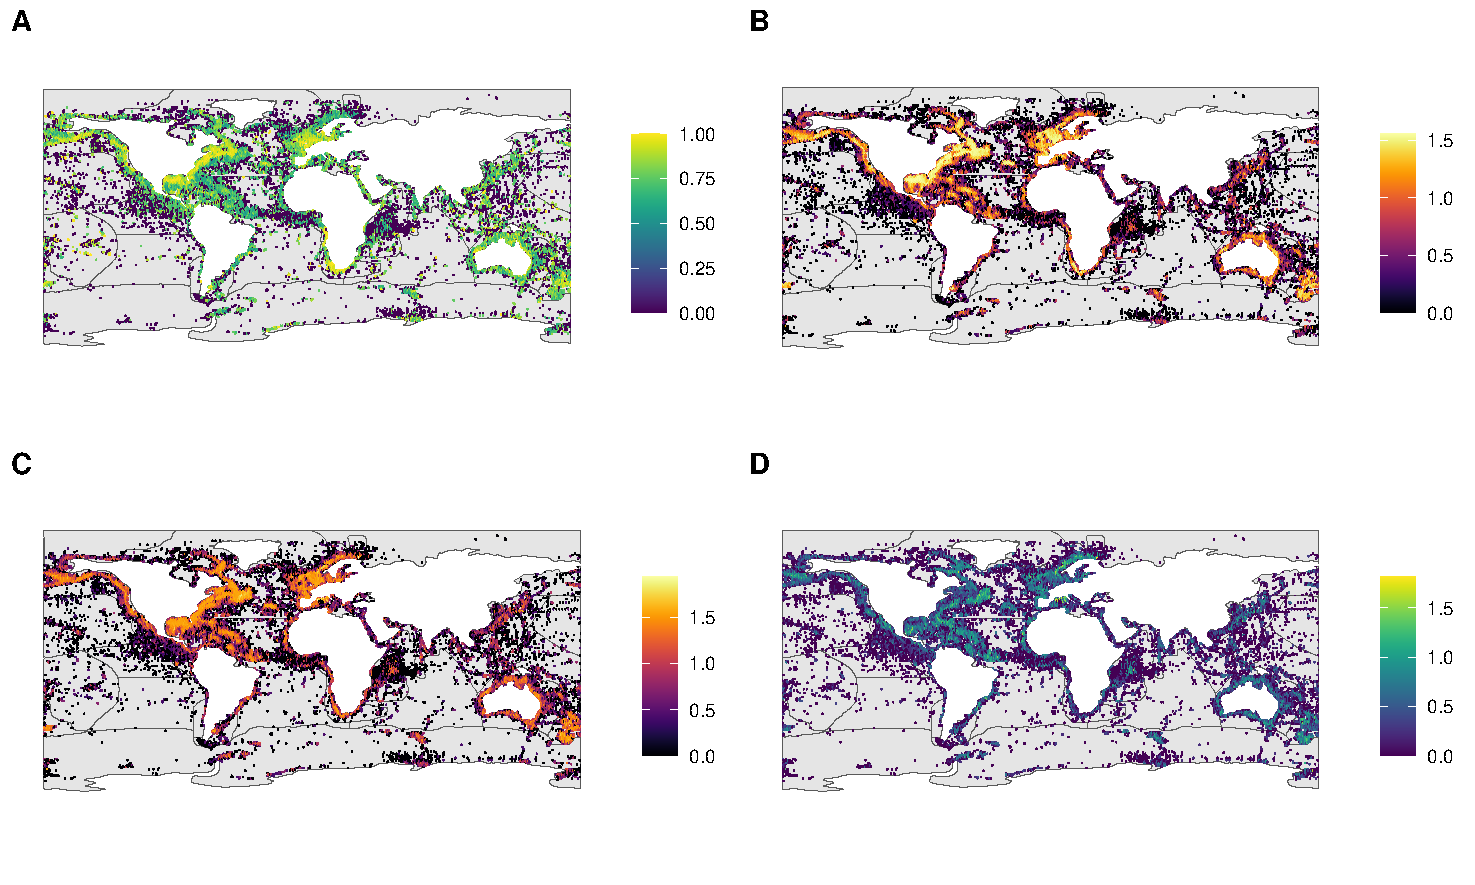
\includegraphics[width=.99\textwidth]{maps_Appendix_2}
    \caption{SRI and Species richness $S$ depicted from GBIF and OBIS databases. \textbf{A}. Species representativeness index; \textbf{B}. Observed species richness ($S_{obs}$); \textbf{C}. Expected species richness ($S_{exp}$); \textbf{D}. Difference between raw estimated and observed richness. The difference has been $log_{10}$ transformed after  subtraction.   \label{fig:S+So+Es}
  }
  
\end{figure}


\section{Grids resolutions}
\label{sec: grids}

For spatial representation analysis we evaluated two additional spatial resolutions (5$^\circ \times$ 5$^\circ$ = 3,021 cells, and 10$^\circ \times$ 10$^\circ$ = 958 cells). Table \ref{tab: percentage} contains the results of this analysis for these grids. We have also mapped these results (see Figure \ref{fig:FigS1}), to understand how the effect of spatial resolution on the evaluation of biodiversity macropatterns. Finally, we also plot the frequency of cells for each SRI category for the three grid sizes (R1=1$^\circ \times$ 1$^\circ$; R5=5$^\circ \times$ 5$^\circ$; R10=10$^\circ \times$ 10$^\circ$) to understand how the data is distributed in our analyses (see Figure \ref{fig:FigS2})


\begin{table}[]
  \centering
  \resizebox{1.0\textwidth}{!}{
\begin{tabular}{|c |c  c  c  c  c | c  c  c  c   c | c  c  c  c  c |}

\hline
   & \multicolumn{5}{| c |} { \textbf{R1} (1$^\circ \times$ 1$^\circ$)} &  \multicolumn{5}{| c |} {\textbf{ R5} (5$^\circ \times$ 5$^\circ$)} & \multicolumn{5}{| c |} { \textbf{R10} (10$^\circ \times$ 10$^\circ$)}\\
 \textbf{ID}  & \textbf{NR} & \textbf{IR} & \textbf{L} & \textbf{M} & \textbf{H} & \textbf{NR} & \textbf{IR} & \textbf{L} & \textbf{M} & \textbf{H} & \textbf{NR} & \textbf{IR} & \textbf{L} & \textbf{M} & \textbf{H} \\ 
  \hline
  \hline
  1  & 18.49 & 15.13 & 5.04 & 36.97 & 24.37 &  0.00 & 16.67 &  0.00 & 33.33 & 50.00 & 16.67 & 16.67 &  0.00 & 33.33 & 33.33 \\ 
  2  & 68.75 & 19.79 & 1.04 & 10.42 &  0.00 & 10.00 & 40.00 & 10.00 & 30.00 & 10.00 & 40.00 &  0.00 &  0.00 & 40.00 & 20.00 \\ 
  3  & 15.74 &  6.54 & 3.39 & 36.80 & 37.53 &  3.57 &  3.37 &  0.00 & 17.86 & 75.00 &  0.00 &  0.00 &  0.00 & 10.00 & 90.00 \\ 
  4  & 46.35 & 22.34 & 7.93 & 22.13 &  1.25 & 28.13 &  9.38 &  6.25 & 40.63 & 15.63 & 30.77 & 15.38 &  0.00 & 23.08 & 30.77 \\ 
  5  & 42.39 & 14.75 & 4.92 & 27.87 & 10.07 & 14.29 &  3.57 &  0.00 & 32.14 & 50.00 & 16.67 &  8.33 &  0.00 &  8.33 & 66.67 \\ 
  6  & 94.96 &  2.21 & 0.13 &  1.87 &  0.83 & 82.13 &  5.64 &  0.31 &  6.58 &  5.33 & 62.65 & 13.25 &  1.20 & 10.84 & 12.05 \\ 
  7  & 63.24 & 11.24 & 0.87 & 14.46 & 10.19 & 17.09 &  9.40 &  3.42 & 29.06 & 41.03 &  7.69 &  7.69 &  2.56 & 35.90 & 46.15 \\ 
  8  & 79.52 & 11.27 & 0.89 &  7.17 &  1.15 & 43.93 & 11.56 &  4.05 & 32.37 &  8.09 & 32.69 & 11.54 &  3.85 & 40.38 & 11.54 \\ 
  9  & 88.74 &  8.71 & 0.00 &  1.57 &  0.99 & 28.74 & 22.99 &  2.87 & 38.51 &  6.90 &  7.69 &  9.62 & 21.15 & 38.08 & 13.46 \\ 
  10 & 96.31 &  2.41 & 0.04 &  0.88 &  0.36 & 70.87 & 15.75 &  0.79 &  7.09 &  5.51 & 51.28 & 15.38 &  2.56 & 20.51 & 10.26 \\ 
  11 & 23.82 &  8.42 & 5.65 & 32.85 & 29.26 &  8.62 &  0.00 &  0.00 & 18.97 & 72.41 &  0.00 & 10.53 &  0.00 &  5.26 & 84.21 \\ 
  12 & 35.59 & 21.61 & 2.45 & 35.59 &  4.76 & 14.29 &  4.76 &  2.38 & 47.62 & 30.95 &  5.88 & 11.76 &  0.00 & 17.65 & 64.71 \\ 
  13 & 67.52 & 15.80 & 1.01 & 12.00 &  3.67 & 13.76 & 12.84 &  7.34 & 44.95 & 21.10 &  9.46 &  6.76 &  2.70 & 44.59 & 36.49 \\ 
  14 & 45.83 & 10.83 & 2.50 & 30.83 & 10.00 & 46.15 &  0.00 &  0.00 &  7.69 & 46.15 & 25.00 &  0.00 &  0.00 &  0.00 & 75.00 \\ 
  15 & 74.52 & 13.06 & 0.00 &  7.07 &  5.35 & 20.00 &  6.67 &  6.67 & 40.00 & 26.67 & 37.50 & 12.50 &  0.00 & 37.50 & 12.50 \\ 
  16 & 36.68 & 10.95 & 3.84 & 34.65 & 13.88 &  5.77 &  7.69 &  3.85 & 28.85 & 53.85 & 10.53 &  0.00 &  0.00 & 21.05 & 68.42 \\ 
  17 & 91.36 &  4.90 & 0.00 &  1.57 &  2.17 & 47.93 & 19.01 &  0.00 & 20.66 & 12.40 & 25.00 &  8.33 &  0.00 & 36.11 & 30.56 \\ 
  18 & 48.29 & 16.27 & 3.78 & 22.06 &  9.61 &  6.50 &  7.32 &  7.32 & 43.09 & 35.77 & 10.26 &  5.13 &  0.00 & 28.21 & 56.41 \\ 
  19 & 90.40 &  6.93 & 0.06 &  2.27 &  0.35 & 53.45 & 18.39 &  3.45 & 17.82 &  6.90 & 31.48 & 12.96 &  1.85 & 35.19 & 18.52 \\ 
  20 & 63.61 & 17.35 & 1.43 & 13.56 &  4.04 &  8.20 &  8.20 &  9.84 & 44.26 & 29.51 & 15.00 &  5.00 &  0.00 & 45.00 & 35.00 \\ 
  21 & 74.78 &  9.63 & 2.84 & 11.48 &  1.27 & 34.68 & 13.51 &  3.15 & 28.38 & 20.27 & 21.21 &  9.09 &  0.00 & 27.27 & 42.42 \\ 
  22 & 76.12 & 18.00 & 0.00 &  5.10 &  0.78 & 33.33 &  6.17 & 16.05 & 43.21 &  1.23 &  9.09 &  4.55 &  9.09 & 59.09 & 18.18 \\ 
  23 & 34.65 & 32.02 & 2.89 & 24.41 &  6.04 & 25.93 &  0.00 & 14.81 & 51.85 &  7.41 &  0.00 & 18.18 &  0.00 & 36.36 & 45.45 \\ 
  24 & 63.07 & 17.89 & 1.38 & 13.53 &  4.13 & 25.93 &  7.41 &  3.70 & 51.85 & 11.11 & 20.00 & 10.00 &  0.00 & 50.00 & 20.00 \\ 
  25 & 88.02 &  4.96 & 0.83 &  5.37 &  0.83 & 52.63 & 10.53 &  0.00 & 21.05 & 15.79 & 42.86 &  0.00 &  0.00 & 28.57 & 28.57 \\ 
  26 & 60.93 &  7.04 & 2.41 & 22.41 &  7.22 & 27.27 & 12.12 &  0.00 & 30.30 & 30.30 & 16.67 &  0.00 &  0.00 & 33.33 & 50.00 \\ 
  27 & 66.84 & 10.35 & 0.70 &  8.07 & 14.04 & 27.78 & 16.67 &  0.00 & 22.22 & 33.33 &  7.69 &  7.69 &  0.00 & 23.08 & 61.54 \\ 
  28 & 59.84 &  9.17 & 2.13 & 17.67 & 11.19 & 30.19 &  7.55 &  1.89 & 30.19 & 30.19 & 30.00 & 10.00 &  0.00 & 25.00 & 35.00 \\ 
  29 & 41.96 & 19.87 & 2.84 & 26.81 &  8.52 & 15.00 & 10.00 &  5.00 & 40.00 & 30.00 & 12.50 & 12.50 &  0.00 & 37.50 & 37.50 \\ 
  30 & 93.74 &  3.49 & 0.20 &  1.97 &  0.59 & 69.45 & 11.02 &  1.00 & 10.52 &  8.01 & 42.29 & 16.57 &  2.86 & 22.29 & 16.00 \\ 
\hline
   \hline
\end{tabular}
}
\caption{
  Surface area as a percentage of each bioregion (ID) for every SRI category for each of the three grid sizes (R1=1$^\circ \times$ 1$^\circ$; R5=5$^\circ \times$ 5$^\circ$; R10=10$^\circ \times$ 10$^\circ$). Values  show the surface area as a percentage of each bioregion for every SRI category (see \S 2.2.1). ID is the identification number given to each bioregion (Table \ref{tab: recuento}). H are cells with a high representativeness of species richness (i.e. SRI $>$ 0.85. M are cells considered as having a medium representativeness (i.e. SRI $\in$ (0.60, 0.85). L cells are cells with a low number of records and are thus not considered to be representative of actual species richness (i.e. SRI $\in$ (0, 0.6)). NR as cells with no records (SRI= \textit{NA}), and IR as cell with insufficient records to apply SRI. \label{tab: percentage} }
\end{table}


\begin{figure}[h]
\centering
\includegraphics[width=.99\textwidth]{Fig_AB_nov}
\caption[]{Spatial representativeness index (SRI) mapping of cells of size: A=5$^\circ \times$ 5$^\circ$; B=10$^\circ \times$ 10$^\circ$. The categorization of the cells corresponds to the level reached by the SRI, where SRI $>$ 0.85: Amount of data is \textit{high} for the representation of species richness (H); SRI=0.60-0.85: Amount of data can be considered of \textit{medium} representativeness (M); SRI=0-0.60: Amount of records is \textit{low} (L); and SRI = NA: cells with no records (NR). IR arecell with \textit{insufficient records} to evaluate species diversity representativeness.
\label{fig:FigS1}}
\end{figure}

\begin{figure}[h]
  \centering
  \includegraphics[width=.8\textwidth]{Fig_B8}
    \caption{Density probability distribution of SRI in three grids of different sizes: R1 = 1$^\circ \times$ 1$^\circ$ (blue line); R5= 5$^\circ \times$ 5$^\circ$ (red line); and R10 = 10$^\circ \times$ 10$^\circ$ (yellow line).
    \label{fig:FigS2}
  }
\end{figure}


\section{Bioregions slopes}
\label{sec:bioregions-slopes}
We evaluated the slopes of the last 10\% of the accumulation curves of each bioregion in our temporal representation analysis. Table \ref{tab:slope} shows the result for each bioregion.

\begin{table}[h]
\centering
\begin{tabular}{| c | r |}
  \hline
\textbf{Bioregion} & \textbf{Slope} \\ 
  \hline
  \hline
1 & 0.35 \\ 
2 & 1.16 \\ 
3 & 1.79 \\ 
4 & 0.91 \\ 
5 & 1.76 \\ 
6 & 0.65 \\ 
7 & 4.44 \\ 
8 & 1.37 \\ 
9 & 6.18 \\ 
10 & 4.87 \\ 
11 & 10.37 \\ 
12 & 7.57 \\ 
13 & 32.86 \\ 
14 & 4.90 \\ 
15 & 6.78 \\ 
16 & 21.62 \\ 
17 & 10.10 \\ 
18 & 6.59 \\ 
19 & 12.44 \\ 
20 & 23.21 \\ 
21 & 11.70 \\ 
22 & 1.85 \\ 
23 & 4.42 \\ 
24 & 3.49 \\ 
25 & 2.12 \\ 
26 & 7.74 \\ 
27 & 12.29 \\ 
28 & 4.82 \\ 
29 & 14.08 \\ 
30 & 2.74 \\ 
  \hline
   \hline
\end{tabular}
\caption{Final slope (10$\%$) of the accumulation curves for each bioregion}
\label{tab:slope}
\end{table}

\section{GAP Analysis}
\label{sec:gap-analysis-1}
We plotted the percentage of surface with marine protected areas of each bioregion (Fig \ref{fig:FigS3}), and the percentage of cells of each FAO Area for each category of SRI value (Fig \ref{fig:FigS4}).

\begin{figure}[h]
  \centering
  \includegraphics[width=1.0\textwidth]{FigS3}
    \caption{Percentage of surface with marine protected areas by bioregions.
    \label{fig:FigS3}
  }
\end{figure}

\begin{figure}[h]
  \centering
  \includegraphics[width=.95\textwidth]{FigS4}
    \caption{Percentage of cells of each FAO Area for each category of SRI value. High representativeness of observed species richness (``H''); SRI=0.60-0.85: Medium representativeness \textit{Sufficient} (``M''); SRI=0-0.60: Low number of records  (``L''); and SRI = NA: cells with no records (``NR'').
    \label{fig:FigS4}
  }
\end{figure}




\end{document}